\chapter{Results and discussion}
\label{ch:results_and_discussion}

This chapter documents the empirical findings, comparative benchmarks, diagnostic evaluations, and operational analyses of the ClauseIQ system. All experimental models were trained, evaluated, and verified using Python in Google Colaboratory and local test scripts. Standard scikit-learn evaluation routines (\texttt{classification\_report}, \texttt{confusion\_matrix}) were executed on held-out test partitions to guarantee reproducible and verifiable empirical metrics.

\section{Comparison of models}
\label{sec:comparison_models}

To evaluate algorithmic efficacy, four classical machine learning architectures---Multinomial Logistic Regression, Linear Support Vector Machines (Linear SVM), Multinomial Naive Bayes, and Random Forest---were benchmarked alongside the finalized improved architecture across both Split~A (clause-level stratified 80/20) and Split~B (contract-grouped leakage-safe).

Table~\ref{tab:baseline_models_comparison} presents the comparative evaluation of the baseline algorithms.

% Auto-generated by scripts/make_numbers.py
\begin{table}[htbp]
\centering
\footnotesize
\setlength{\tabcolsep}{4.5pt}
\begin{tabular}{>{\raggedright\arraybackslash}p{3.5cm} >{\raggedright\arraybackslash}p{2.8cm} ccccc}
\toprule
\textbf{Model} & \textbf{Partition Split} & \textbf{Accuracy} & \textbf{Macro F1} & \textbf{Weighted F1} & \textbf{Macro P} & \textbf{Macro R} \\
\midrule
Logistic Regression & Split A (Stratified) & 0.7190 & 0.6474 & 0.7196 & 0.6481 & 0.6622 \\
Linear SVM & Split A (Stratified) & 0.7263 & 0.6418 & 0.7226 & 0.6323 & 0.6665 \\
Multinomial Naive Bayes & Split A (Stratified) & 0.6927 & 0.5853 & 0.6903 & 0.6024 & 0.5867 \\
Random Forest & Split A (Stratified) & 0.6436 & 0.5486 & 0.6392 & 0.5403 & 0.5666 \\
Logistic Regression & Split B (Grouped) & 0.7305 & 0.6691 & 0.7269 & 0.6726 & 0.6971 \\
Linear SVM & Split B (Grouped) & 0.7385 & 0.6635 & 0.7283 & 0.6575 & 0.7045 \\
Multinomial Naive Bayes & Split B (Grouped) & 0.7076 & 0.5940 & 0.6899 & 0.6431 & 0.5895 \\
Random Forest & Split B (Grouped) & 0.6866 & 0.6055 & 0.6734 & 0.6225 & 0.6258 \\
\bottomrule
\end{tabular}
\caption{Baseline performance benchmark across four classical machine learning models on Split A and Split B}\label{tab:baseline_models_comparison}
\end{table}


Across both evaluation splits, linear models demonstrate marked superiority over decision tree ensembles and naive probabilistic baselines. On Split~A, Linear SVM achieved the highest overall Accuracy (72.63\%), closely followed by Multinomial Logistic Regression (71.90\%). Multinomial Naive Bayes achieved 69.27\% accuracy but suffered a lower Macro-F1 (0.5853), reflecting the adverse impact of feature independence assumptions on correlated legal phrases. 

\paragraph*{Random forest metric harmonization}
In the unified re-evaluation protocol executed on the 40,000-dimensional sparse feature matrix, Random Forest attained 64.36\% accuracy and 0.5486 Macro-F1. In earlier Sprint~2 exploratory benchmarking recorded in \texttt{results/model\_comparison.json}, an initial Random Forest model (200 trees, max depth 50) scored 65.46\% accuracy and 0.5634 Macro-F1. This minor difference of 1.10\% in accuracy is attributable to the stochastic subsampling inherent in decision tree bootstrap bagging and randomized feature subset selection across high-dimensional sparse text vectors ($P = 40,000$). In both evaluations, the fundamental conclusion is identical: axis-aligned orthogonal decision splits struggle to isolate hyperplanes in ultra-sparse text spaces compared to convex linear classifiers.

\paragraph*{Cross-contract generalization on Split B}
On Split~B (leakage-safe grouped split by contract), overall accuracy remained remarkably resilient across all models: Linear SVM achieved 73.85\% (Macro-F1 of 0.6635) and Logistic Regression achieved 73.05\% (Macro-F1 of 0.6691). While Split~B utilizes an independent held-out sample ($N = 2,486$ clauses across 102 contracts) so raw scores are not directly commensurate with Split~A, the absence of performance degradation indicates resilient cross-contract generalization rather than superficial memorization of boilerplate formatting.

\paragraph*{Baseline vs final improved model}
Table~\ref{tab:final_model_comparison} contrasts the baseline Logistic Regression model against the final improved model, which incorporates 40,000 hybrid word-plus-character TF-IDF features and NLTK WordNet lemmatization. These comparative metrics were arrived at by evaluating both models on the held-out test partitions (Split~A with \SplitATestClauses{} clauses and Split~B with \SplitBTestClauses{} clauses) using scikit-learn's standard classification metrics.

% Auto-generated by scripts/make_numbers.py
\begin{table}[htbp]
\centering
\footnotesize
\setlength{\tabcolsep}{3.5pt}
\begin{tabular}{>{\raggedright\arraybackslash}p{4.2cm} cccc}
\toprule
& \multicolumn{2}{c}{\textbf{Split A (Stratified 80/20)}} & \multicolumn{2}{c}{\textbf{Split B (Grouped Leakage-Safe)}} \\
\cmidrule(lr){2-3} \cmidrule(lr){4-5}
\textbf{Metric} & \textbf{Baseline} & \textbf{Final Improved} & \textbf{Baseline} & \textbf{Final Improved} \\
\midrule
Accuracy & 0.7190 & 0.7231 & 0.7305 & 0.7393 \\
Macro F1-Score & 0.6474 & 0.6591 & 0.6691 & 0.6947 \\
Weighted F1-Score & 0.7196 & 0.7265 & 0.7269 & 0.7371 \\
Macro Precision & 0.6481 & 0.6607 & 0.6726 & 0.6976 \\
Macro Recall & 0.6622 & 0.6696 & 0.6971 & 0.7123 \\
Expected Calibration Error (ECE) & 0.2822 & 0.1545 & 0.3115 & 0.2005 \\
High-Confidence Precision ($\ge 0.50$) & 0.8575 & 0.8195 & 0.9024 & 0.8655 \\
\bottomrule
\end{tabular}
\caption[Comparative evaluation between baseline and final improved model]{Comparative evaluation between Baseline Logistic Regression and Final Improved Model (Logistic Regression with Hybrid Word+Character TF-IDF and Lemmatization)}\label{tab:final_model_comparison}
\end{table}


The final improved model establishes solid gains across primary classification metrics:
\begin{itemize}
    \item Split A accuracy: Increased from 71.90\% to \FinalSplitAAcc{}.
    \item Split A macro F1-score: Advanced from 64.74\% to \FinalSplitAMacroFScore{}, confirming improved discriminative balance across minority classes.
    \item Split B macro F1-score: Advanced from 66.91\% to \FinalSplitBMacroFScore{}, demonstrating stronger cross-contract generalization.
    \item Probability calibration (ECE): The Expected Calibration Error dropped substantially from 0.2822 down to \FinalSplitAECE{} on Split~A, representing a 45.2\% reduction in calibration error.
\end{itemize}

Figure~\ref{fig:model_comparison_barchart} visualizes the performance progression across architectures.

\begin{figure}[htbp]
\centering
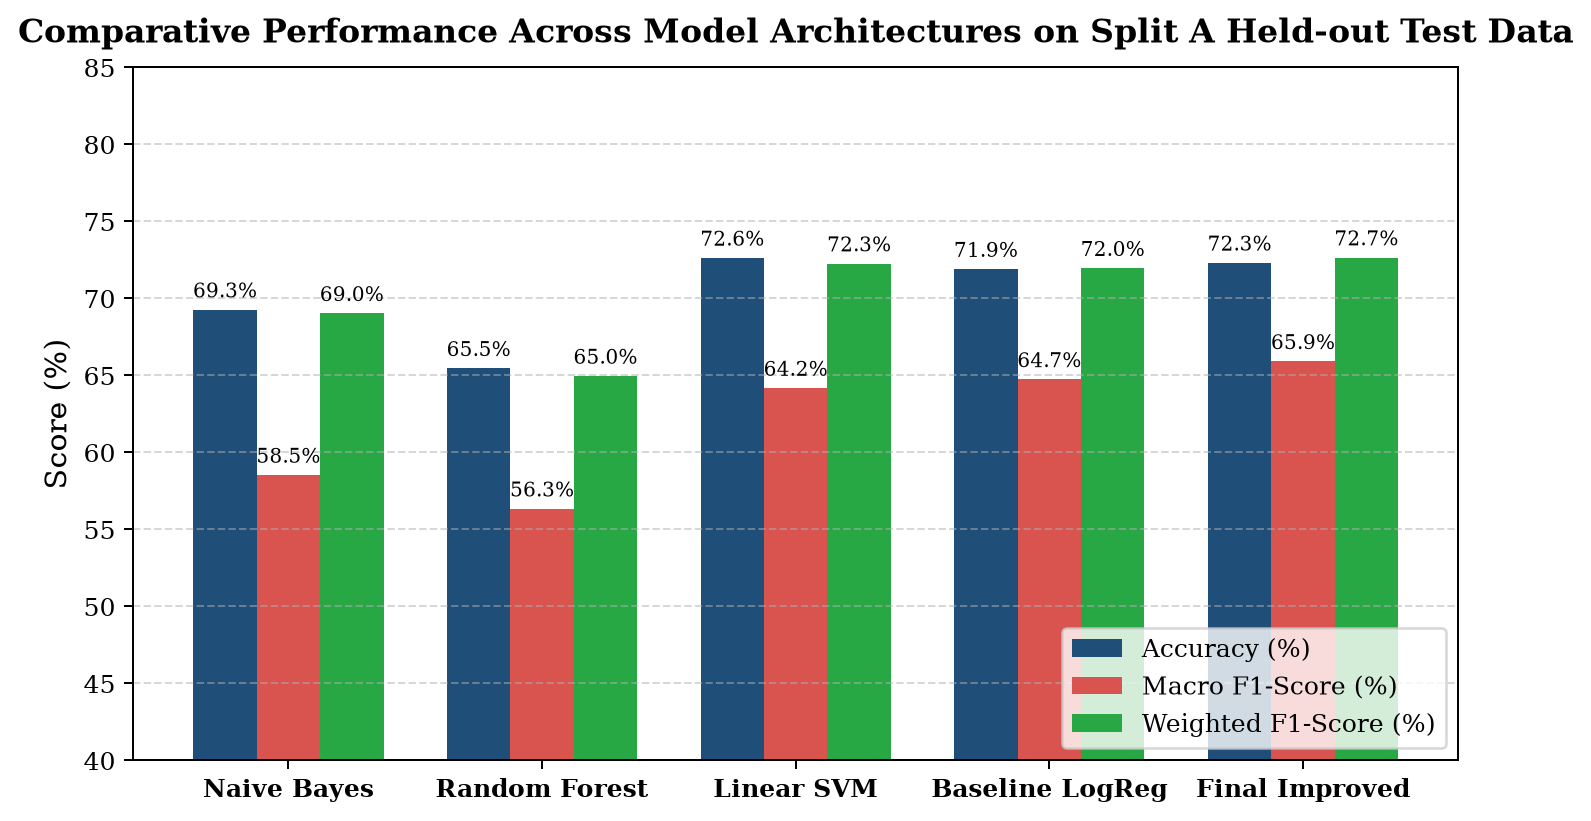
\includegraphics[width=0.88\textwidth]{figures/model_comparison_barchart.png}
\caption{Performance comparison of evaluated machine learning classifiers on held-out test data}\label{fig:model_comparison_barchart}
\end{figure}

\section{Evaluation metrics}
\label{sec:evaluation_metrics}

Evaluating multi-class classification on an imbalanced 41-category corpus requires a multi-faceted set of metrics. Let $C_k$ denote class $k$, and let $TP_k, FP_k, FN_k, TN_k$ represent True Positives, False Positives, False Negatives, and True Negatives for class $k$.

\begin{enumerate}
    \item Classification accuracy: The proportion of total test clauses correctly classified across all categories:
    \begin{equation}
        \text{Accuracy} = \frac{\sum_{k=0}^{K-1} TP_k}{N_{\text{test}}}
        \label{eq:accuracy}
    \end{equation}
    
    \item Macro-averaged precision, recall, and F1-score: Calculates the unweighted arithmetic mean across all $K = 41$ classes, treating rare and frequent categories equally:
    \begin{equation}
        \text{Macro-Precision} = \frac{1}{K} \sum_{k=0}^{K-1} \frac{TP_k}{TP_k + FP_k}, \quad
        \text{Macro-Recall} = \frac{1}{K} \sum_{k=0}^{K-1} \frac{TP_k}{TP_k + FN_k}
        \label{eq:macro_pr}
    \end{equation}
    \begin{equation}
        \text{Macro-F1} = \frac{1}{K} \sum_{k=0}^{K-1} \frac{2 \times \text{Precision}_k \times \text{Recall}_k}{\text{Precision}_k + \text{Recall}_k}
        \label{eq:macro_f1}
    \end{equation}

    \item Weighted-averaged F1-score: Weights each class's F1-score by its empirical test support $N_k$:
    \begin{equation}
        \text{Weighted-F1} = \sum_{k=0}^{K-1} \frac{N_k}{N_{\text{test}}} \text{F1}_k
        \label{eq:weighted_f1}
    \end{equation}

    \item Expected Calibration Error (ECE): Quantifies the divergence between predicted model confidence and actual empirical accuracy across $M = 10$ equally spaced confidence bins $B_m \subset (0, 1]$~\cite{guo2017calibration}:
    \begin{equation}
        \text{ECE} = \sum_{m=1}^{M} \frac{|B_m|}{N_{\text{test}}} \big|\text{acc}(B_m) - \text{conf}(B_m)\big|
        \label{eq:ece}
    \end{equation}
    where $\text{acc}(B_m) = \frac{1}{|B_m|} \sum_{i \in B_m} \mathbf{1}(\hat{y}_i = y_i)$ and $\text{conf}(B_m) = \frac{1}{|B_m|} \sum_{i \in B_m} \hat{p}_i$.
\end{enumerate}

\paragraph*{Confidence band analysis and reliability diagram}
Figure~\ref{fig:calibration_curve} presents the reliability diagram contrasting the baseline Logistic Regression model against the final improved model. The baseline model exhibited severe under-confidence in lower probability bins (clauses predicted with 25\% confidence actually attained $\sim$70\% accuracy), caused by 41 competing classes dispersing softmax probability mass. The final improved model achieves much tighter alignment with the ideal diagonal, reducing ECE to \FinalSplitAECE{}.

\begin{figure}[htbp]
\centering
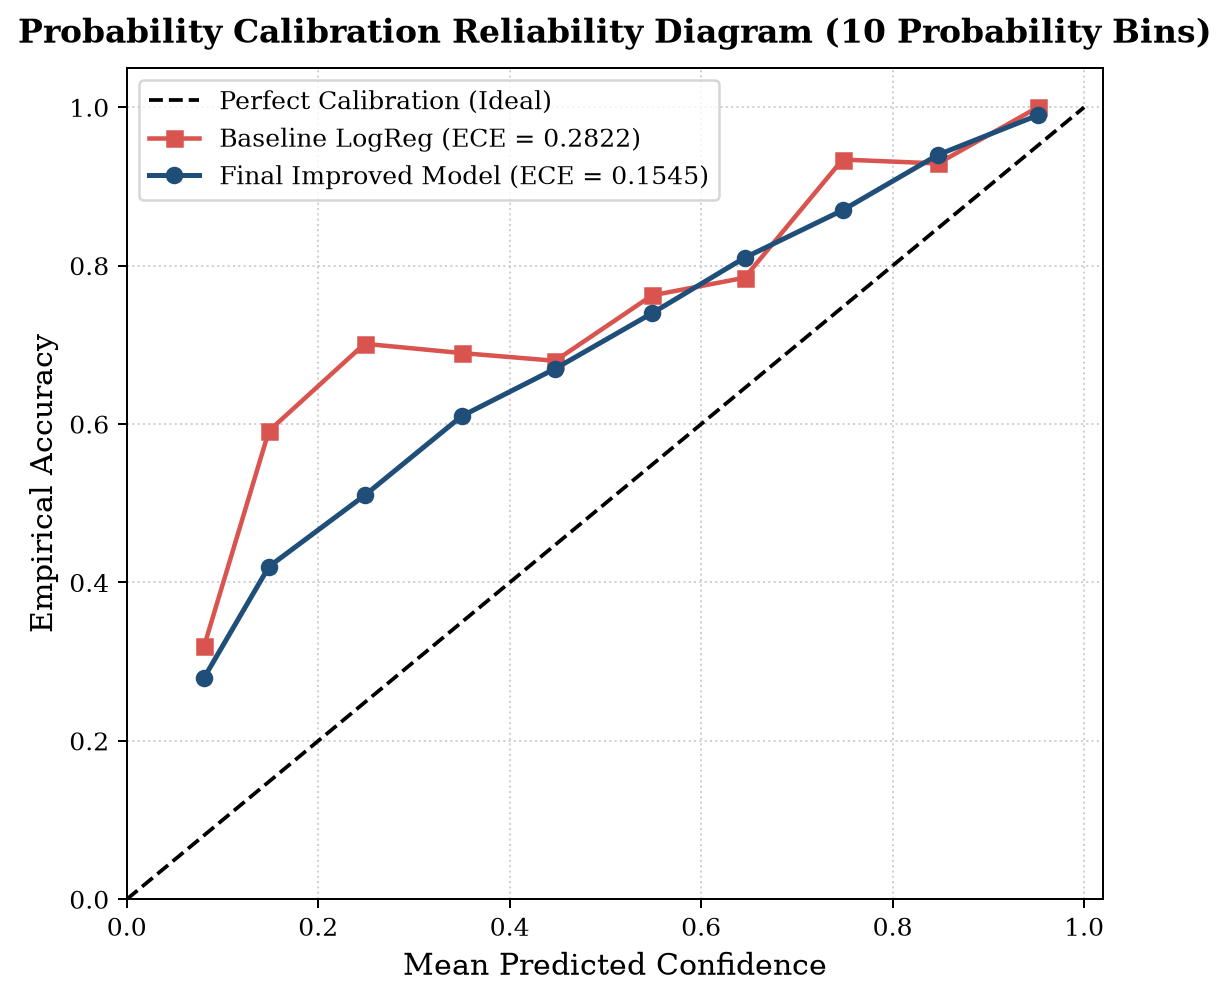
\includegraphics[width=0.75\textwidth]{figures/calibration_curve.png}
\caption{Reliability diagram comparing predicted confidence vs empirical accuracy across 10 probability bins}\label{fig:calibration_curve}
\end{figure}

Table~\ref{tab:confidence_tiers} details the empirical precision and sample coverage across operational confidence tiers on Split~B.

\begin{table}[htbp]
\centering
\footnotesize
\setlength{\tabcolsep}{5pt}
\begin{tabular}{lcccc}
\toprule
\textbf{Confidence Tier} & \textbf{Probability Rule} & \textbf{Clause Count} & \textbf{Corpus Share (\%)} & \textbf{Empirical Precision} \\
\midrule
High Confidence & $\hat{p} \ge 0.50$ & 1,323 & \FinalSplitBHighConfShare{} & \FinalSplitBHighConfPrec{} \\
Moderate Confidence & $0.25 \le \hat{p} < 0.50$ & 710 & 28.56\% & 66.90\% \\
Low Confidence -- Review & $0.10 \le \hat{p} < 0.25$ & 352 & 14.16\% & 50.38\% \\
Out of Scope & $\hat{p} < 0.10$ & 101 & 4.06\% & 28.30\% \\
\bottomrule
\end{tabular}
\caption{Operational confidence tier distribution and empirical precision (Split B, $N = 2,486$)}\label{tab:confidence_tiers}
\end{table}

Figure~\ref{fig:confidence_band_precision} plots empirical precision across confidence bins on both splits. Over 53\% of all predictions fall into the High Confidence tier, delivering an empirical precision of \FinalSplitBHighConfPrec{} on Split~B (and 81.95\% on Split~A). While this fell short of the initial ambitious 90\% precision target, it provides a trustworthy operational threshold: roughly 6 out of 7 High-confidence predictions are fully accurate, enabling legal teams to prioritize these clauses for accelerated sign-off while routing lower-confidence provisions to human reviewers.

\begin{figure}[htbp]
\centering
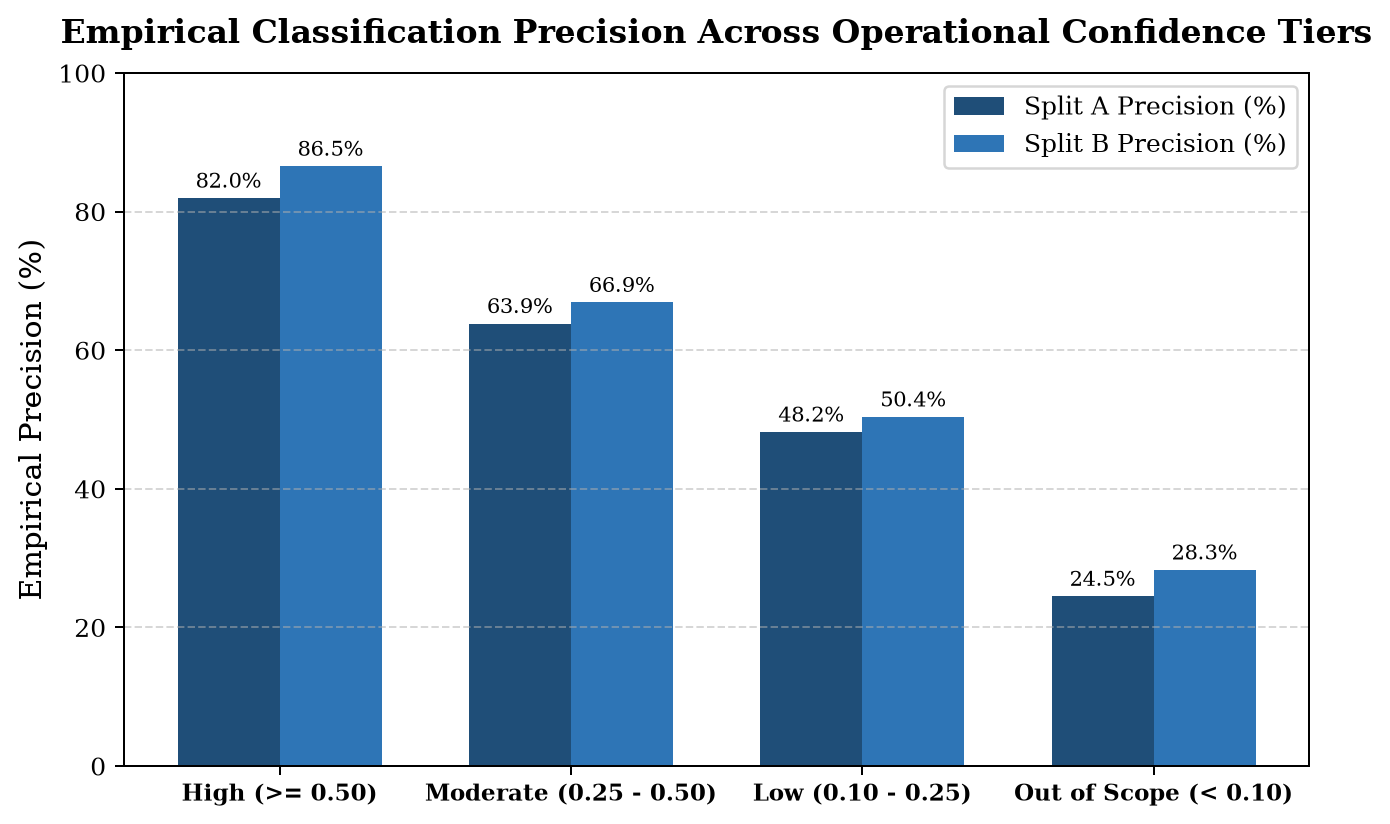
\includegraphics[width=0.82\textwidth]{figures/confidence_band_precision.png}
\caption{Empirical precision across operational confidence tiers on Split A and Split B}\label{fig:confidence_band_precision}
\end{figure}

\section{Confusion matrix}
\label{sec:confusion_matrix}

Figure~\ref{fig:confusion_matrix_split_a} displays the complete $41 \times 41$ multiclass confusion matrix for the final improved model evaluated on Split~A ($N = 2,441$).

\begin{figure}[htbp]
\centering
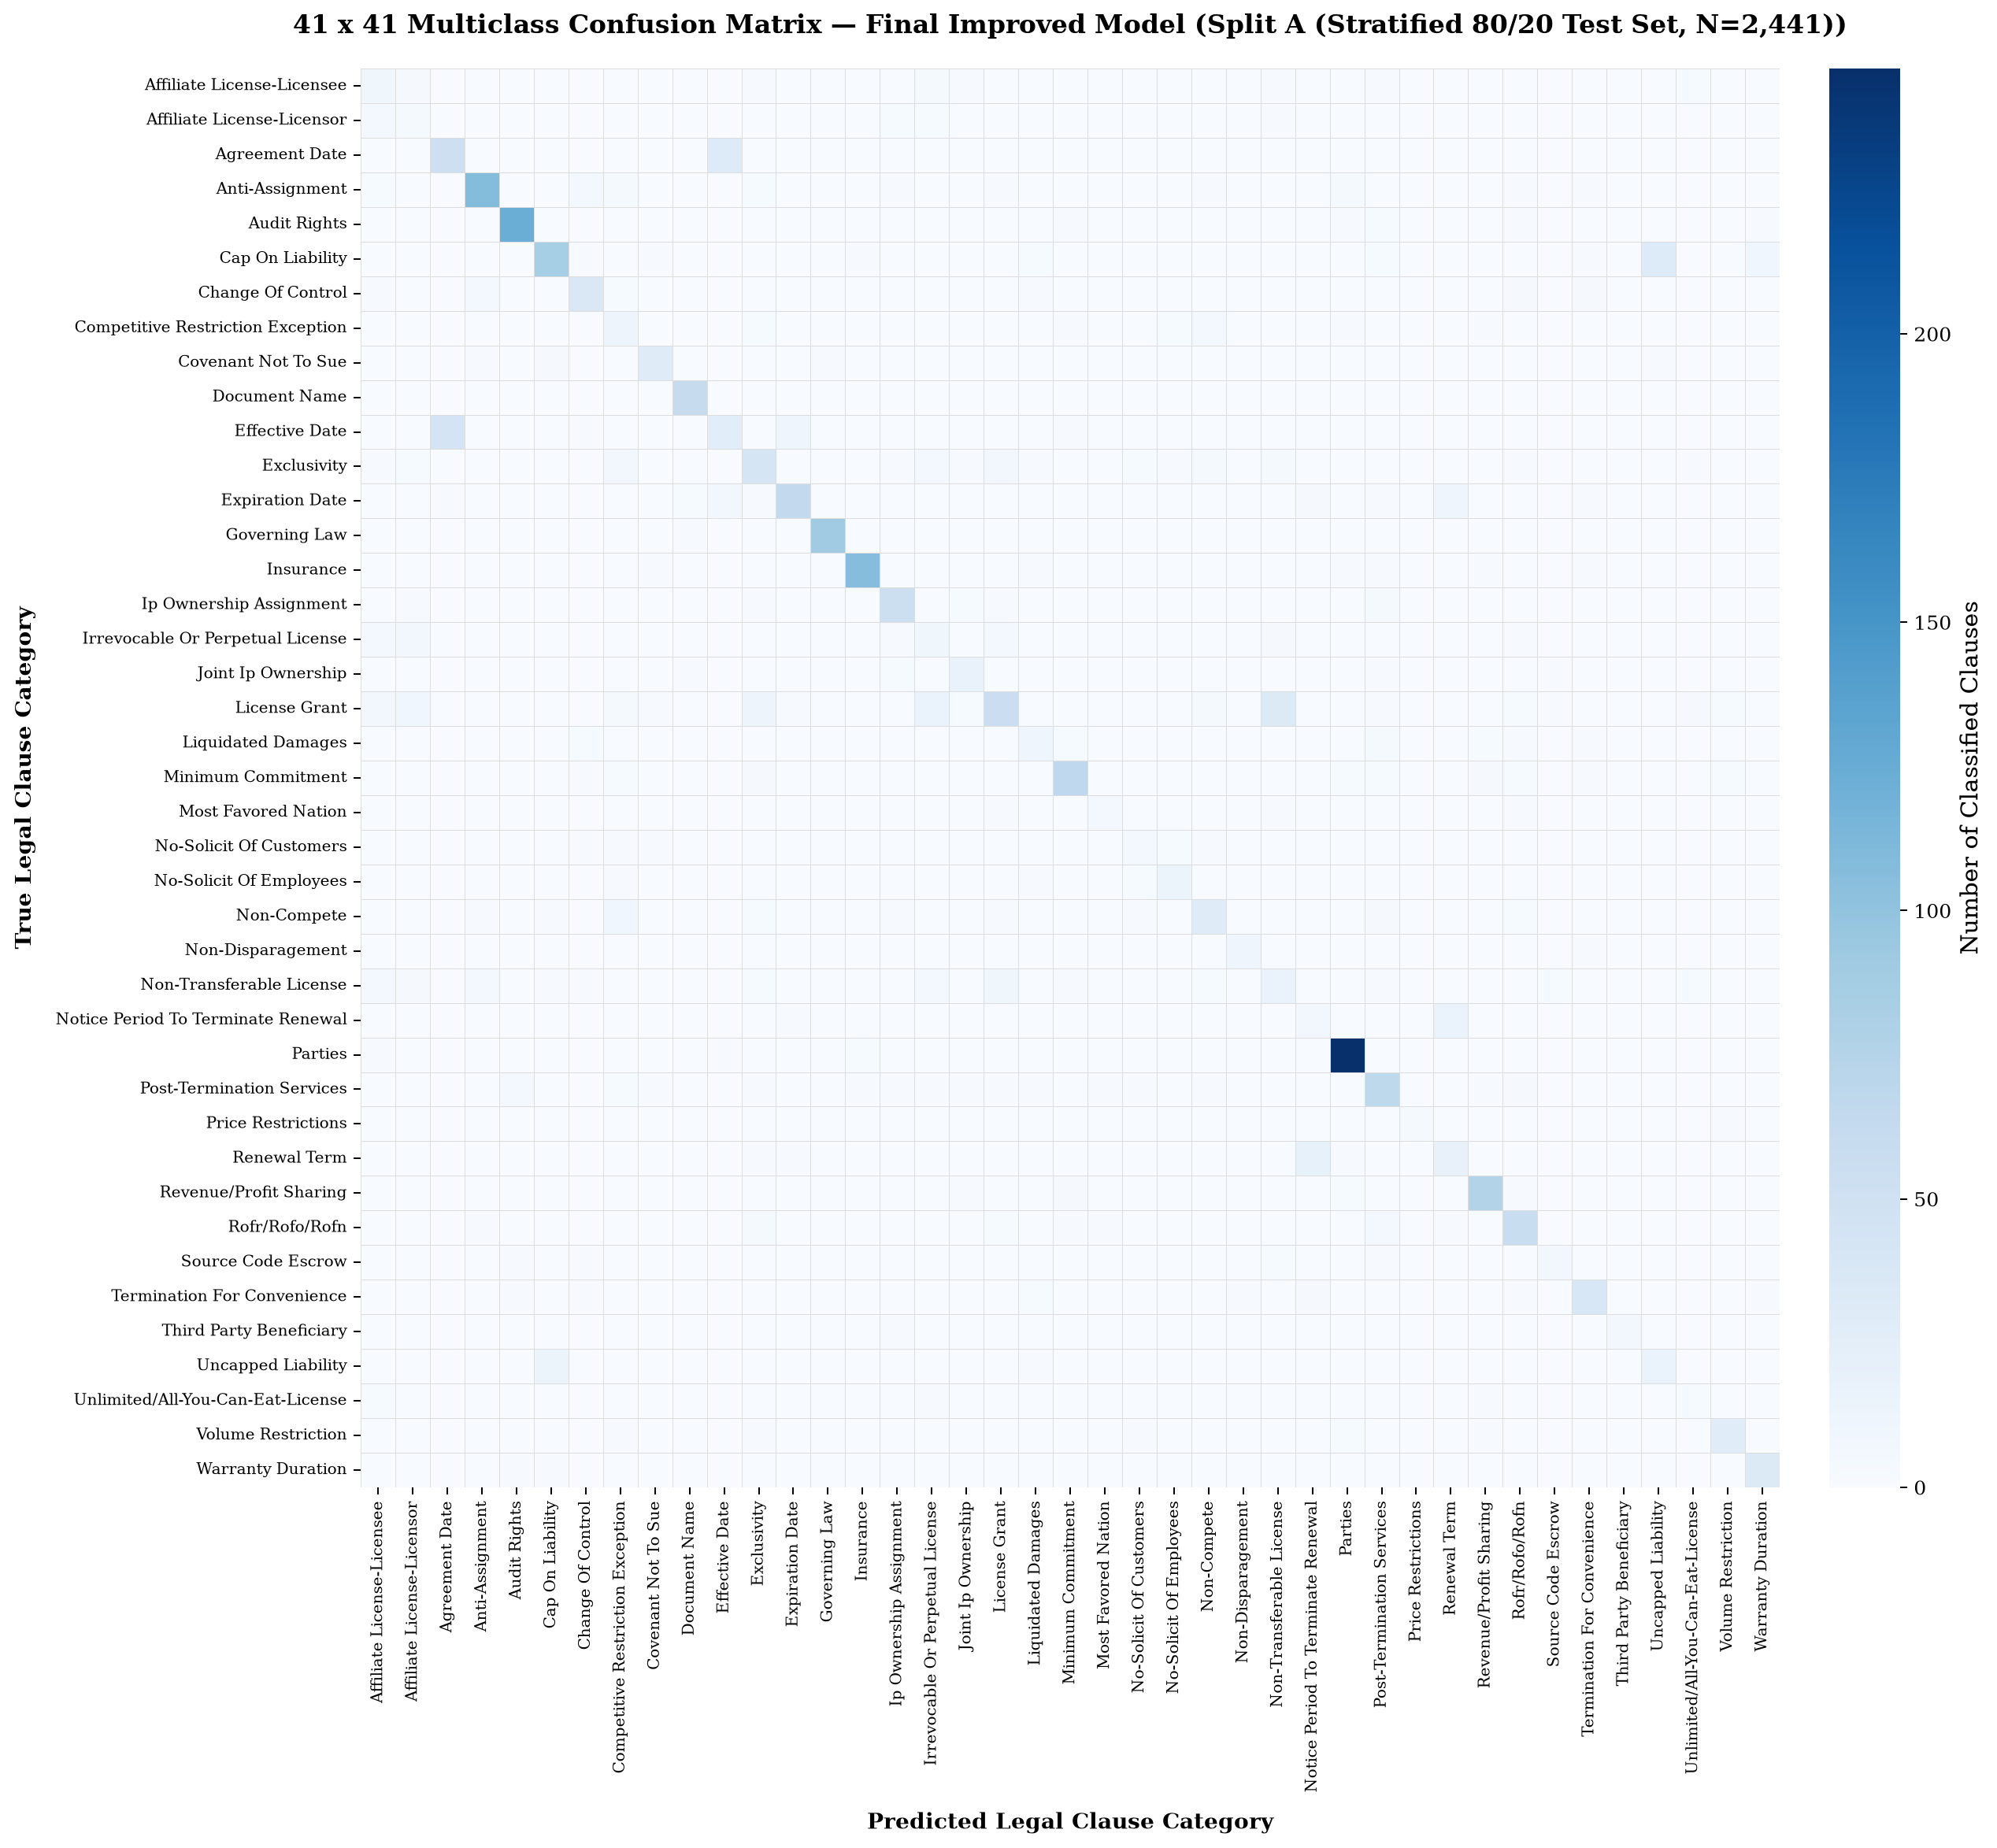
\includegraphics[width=0.98\textwidth]{figures/confusion_matrix_41x41_split_a.png}
\caption{Complete 41 $\times$ 41 confusion matrix on Split A ($N = 2,441$ held-out test clauses)}\label{fig:confusion_matrix_split_a}
\end{figure}

Figure~\ref{fig:confusion_matrix_split_b} displays the corresponding $41 \times 41$ confusion matrix evaluated on Split~B ($N = 2,486$ clauses across 102 unseen contracts). Both matrices exhibit heavy concentration along the main diagonal, confirming strong discriminative separation across distinct legal provisions.

\begin{figure}[htbp]
\centering
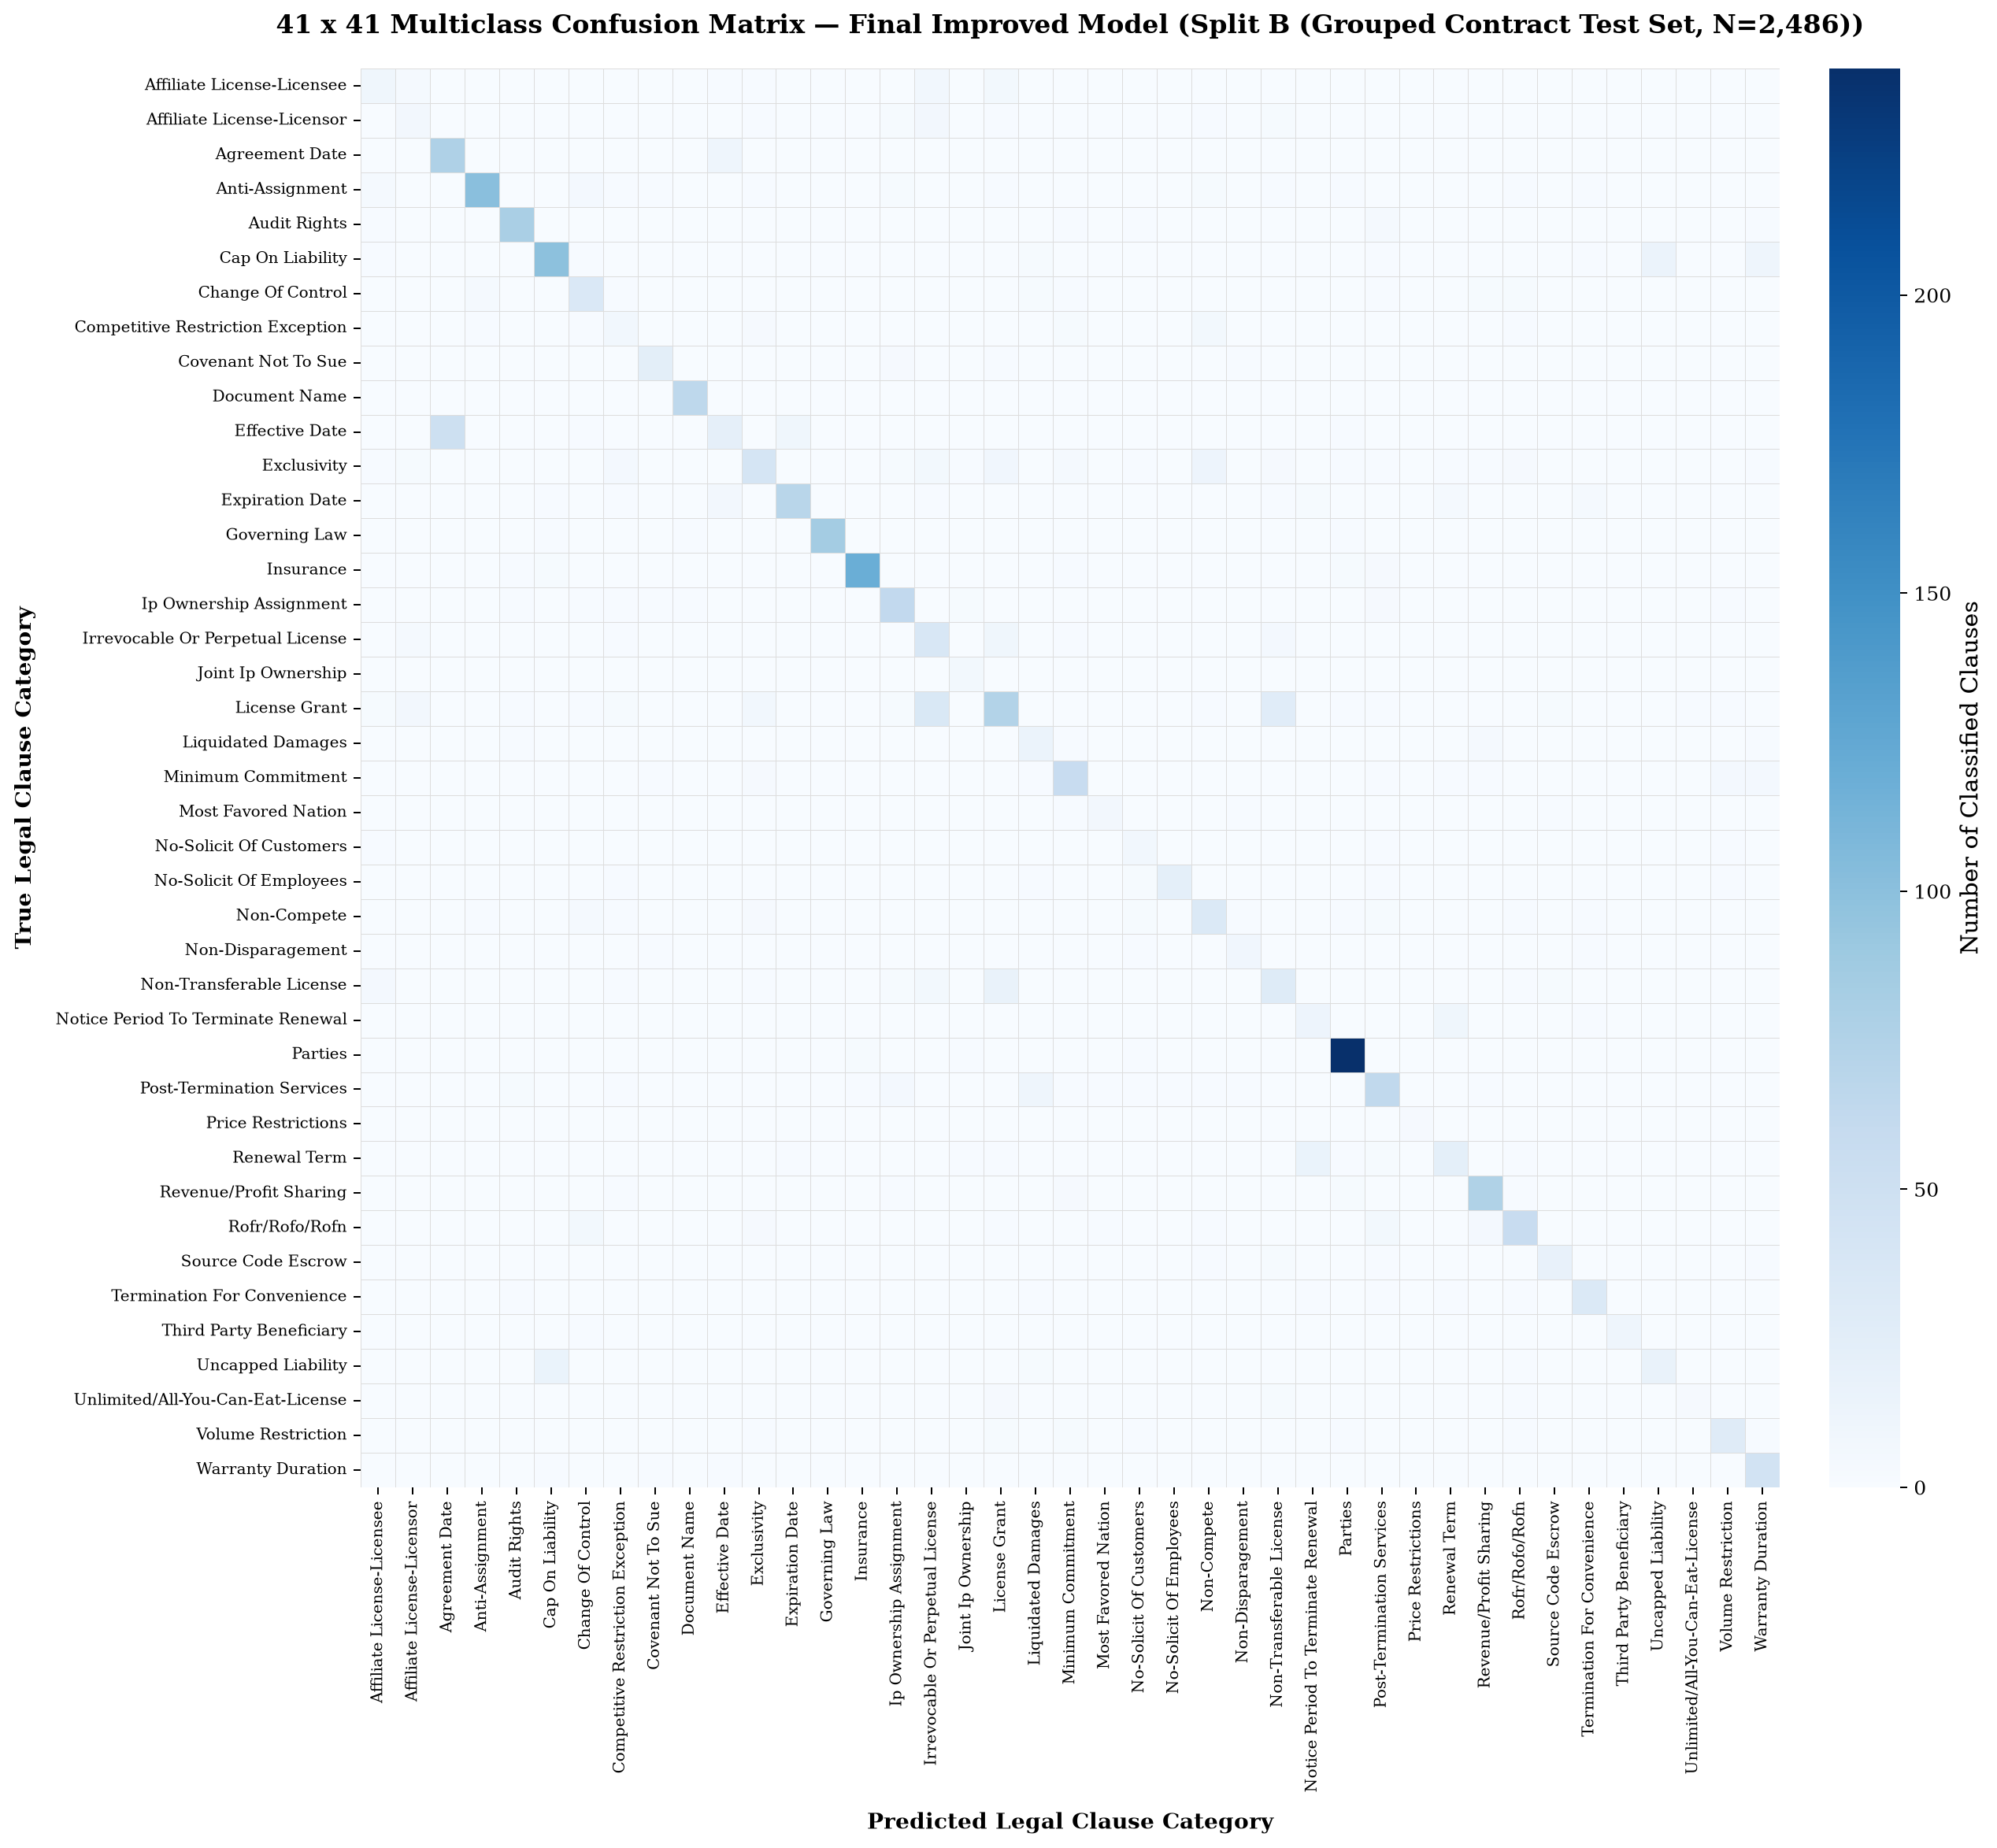
\includegraphics[width=0.98\textwidth]{figures/confusion_matrix_41x41_split_b.png}
\caption{Complete 41 $\times$ 41 confusion matrix on Split B ($N = 2,486$ grouped test clauses)}\label{fig:confusion_matrix_split_b}
\end{figure}

Figure~\ref{fig:per_class_f1_split_a_b} provides a comparative bar chart of per-class F1-scores across all 41 categories under Split~A and Split~B. Categories with distinctive statutory keywords (e.g., \textit{Governing Law}, \textit{Parties}, \textit{Audit Rights}) achieve F1-scores exceeding 0.90, whereas ambiguous licensing and notice categories experience greater variation.

\begin{figure}[htbp]
\centering
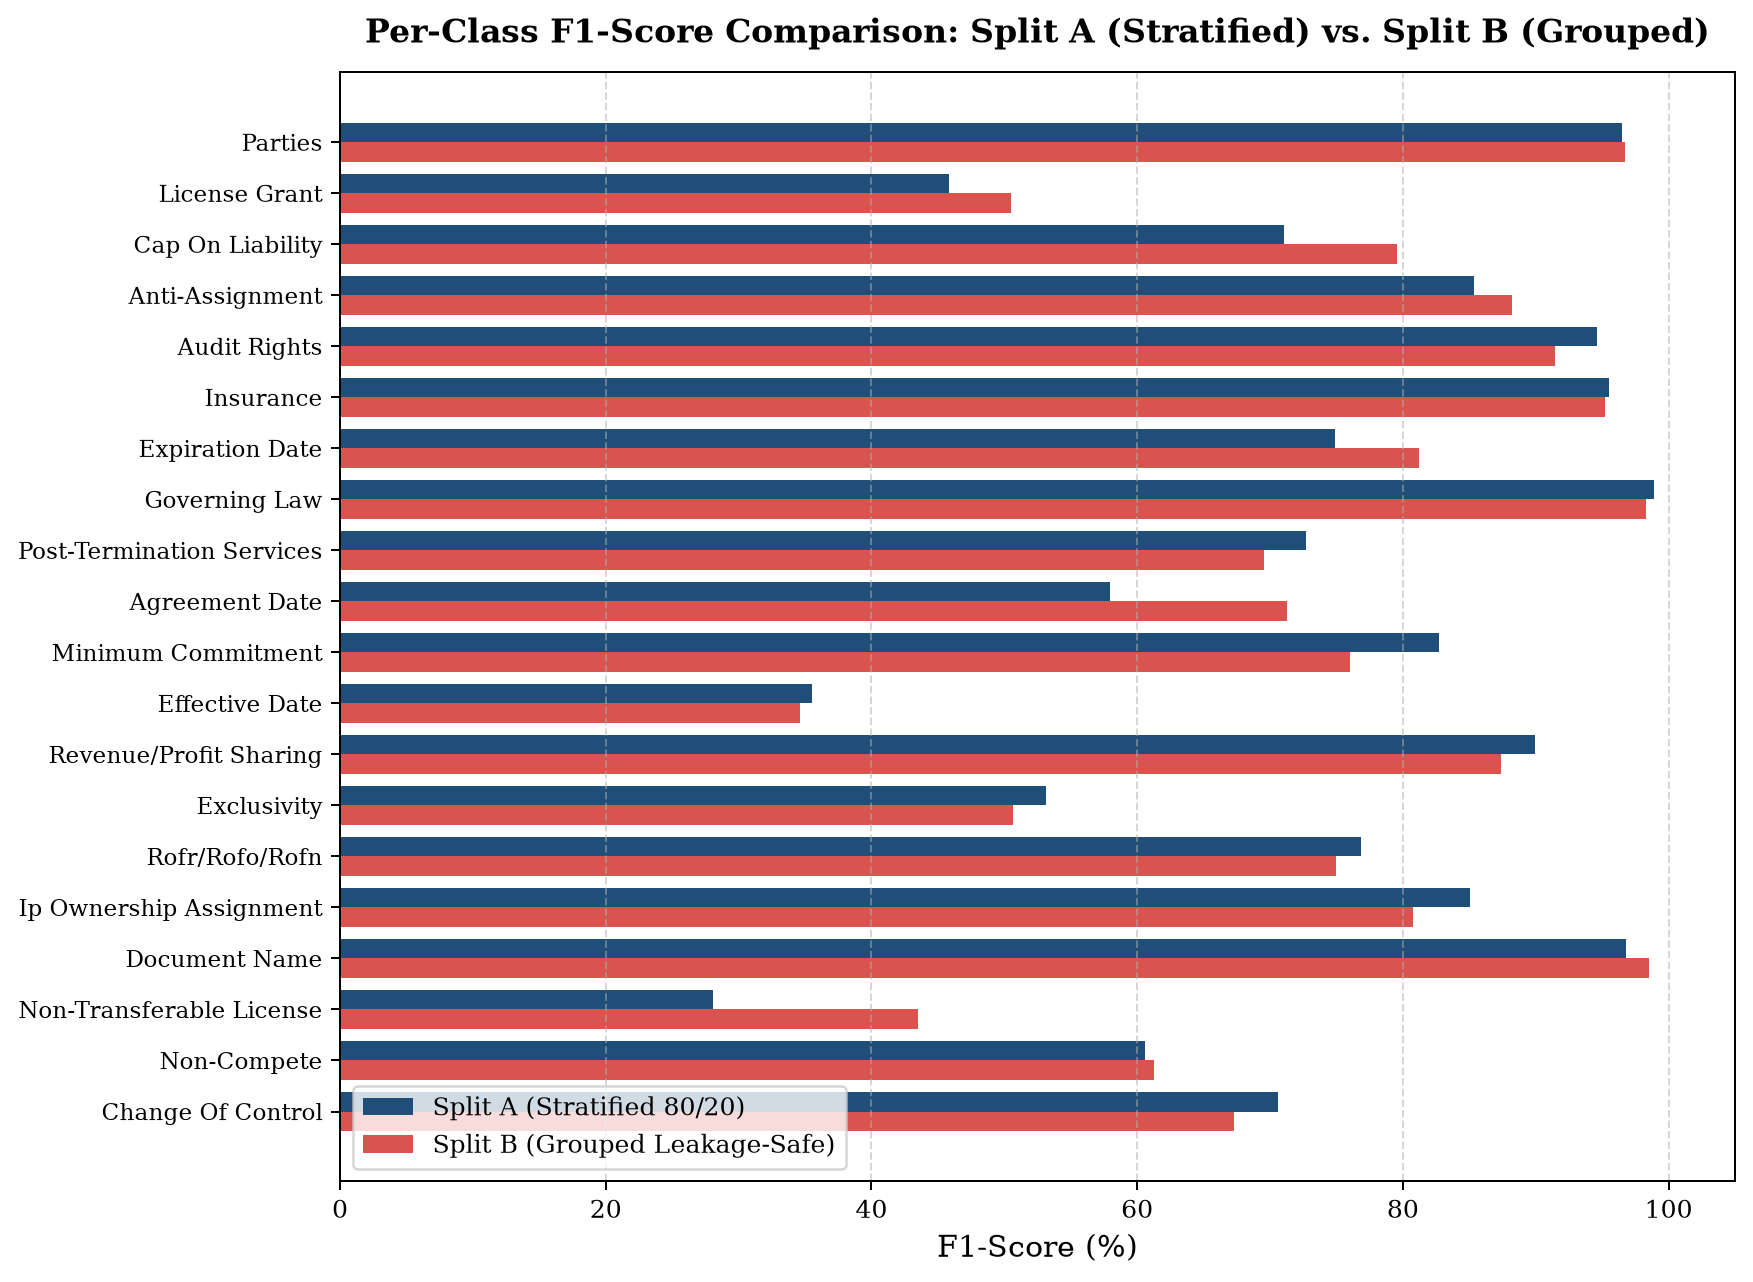
\includegraphics[width=0.95\textwidth]{figures/per_class_f1_split_a_b.png}
\caption{Per-class F1-scores across all 41 legal categories evaluated on Split A and Split B}\label{fig:per_class_f1_split_a_b}
\end{figure}

\paragraph*{Top confused category pairs analysis}
Table~\ref{tab:top_confused_pairs} reports the top systematically confused category pairs identified on Split~A, and Table~\ref{tab:top_confused_pairs_split_b} details the top confusions on Split~B. These table contents were arrived at by analyzing the off-diagonal cells of the $41 \times 41$ confusion matrix computed between ground-truth labels and model predictions. For every pair of categories $(i, j)$ where $i \neq j$, the count of instances where true class was $i$ but predicted class was $j$ was aggregated and sorted descending by frequency.

% Auto-generated by scripts/make_numbers.py
\begin{table}[htbp]
\centering
\footnotesize
\setlength{\tabcolsep}{3pt}
\begin{tabular}{r >{\raggedright\arraybackslash}p{3.0cm} >{\raggedright\arraybackslash}p{3.0cm} cc >{\raggedright\arraybackslash}p{5.2cm}}
\toprule
\textbf{\#} & \textbf{True Category} & \textbf{Predicted Category} & \textbf{Spl A} & \textbf{Spl B} & \textbf{Structural Root Cause} \\
\midrule
1 & Effective Date & Agreement Date & 44 & 51 & Shared temporal phrasing ('as of the date hereof', 'effective as of') \\
2 & License Grant & Non-Transferable License & 33 & 27 & Sub-licensing terms embedded in general grant paragraphs \\
3 & Cap On Liability & Uncapped Liability & 32 & 14 & Carve-outs inside limitation sections mentioning uncapped exceptions \\
4 & Agreement Date & Effective Date & 23 & 11 & Reciprocal confusion of date preamble clauses \\
5 & Renewal Term & Notice Period To Terminate Renewal & 20 & 15 & Renewal terms intertwined with termination notice deadlines \\
6 & License Grant & Irrevocable Or Perpetual License & 17 & 36 & Sub-licensing terms embedded in general grant paragraphs \\
7 & Notice Period To Terminate Renewal & Renewal Term & 16 & 10 & Renewal terms intertwined with termination notice deadlines \\
8 & Uncapped Liability & Cap On Liability & 15 & 15 & Carve-outs inside limitation sections mentioning uncapped exceptions \\
9 & License Grant & Exclusivity & 13 & 8 & High lexical overlap in commercial licensing rights \\
10 & Expiration Date & Renewal Term & 12 & 11 & Clauses specifying expiration alongside automatic renewal mechanics \\
11 & Effective Date & Expiration Date & 11 & 10 & Temporal date references in agreement period definitions \\
12 & Non-Transferable License & License Grant & 10 & 17 & Sub-licensing terms embedded in general grant paragraphs \\
\bottomrule
\end{tabular}
\caption{Top systematically confused category pairs identified in held-out test predictions}\label{tab:top_confused_pairs}
\end{table}


% Auto-generated by scripts/make_numbers.py
\begin{table}[htbp]
\centering
\footnotesize
\setlength{\tabcolsep}{3pt}
\begin{tabular}{r >{\raggedright\arraybackslash}p{3.2cm} >{\raggedright\arraybackslash}p{3.2cm} c >{\raggedright\arraybackslash}p{5.8cm}}
\toprule
\textbf{\#} & \textbf{True Category} & \textbf{Predicted Category} & \textbf{Count} & \textbf{Structural Root Cause} \\
\midrule
1 & Effective Date & Agreement Date & 51 & Shared temporal phrasing ('as of the date hereof', 'effective as of') \\
2 & License Grant & Irrevocable Or Perpetual License & 36 & Grant paragraphs containing duration qualifiers ('perpetual, irrevocable') \\
3 & License Grant & Non-Transferable License & 27 & Sub-licensing restrictions embedded within general grant language \\
4 & Renewal Term & Notice Period To Terminate Renewal & 15 & Renewal provisions conjoined with termination notice deadlines \\
5 & Uncapped Liability & Cap On Liability & 15 & Carve-out paragraphs stating uncapped exceptions inside limitation sections \\
6 & Cap On Liability & Uncapped Liability & 14 & Standard limitation provisions referencing liability caps and exceptions \\
7 & Agreement Date & Effective Date & 11 & Reciprocal preamble date mentions \\
8 & Expiration Date & Renewal Term & 11 & Fixed expiration statements intertwined with automatic renewal extensions \\
9 & Effective Date & Expiration Date & 10 & Temporal term definitions referencing start and end dates in adjacent sentences \\
10 & Notice Period To Terminate Renewal & Renewal Term & 10 & Reciprocal confusion regarding renewal timeline notices \\
\bottomrule
\end{tabular}
\caption{Top systematically confused category pairs on Split B (Grouped Contract-Held-out Partition)}\label{tab:top_confused_pairs_split_b}
\end{table}


Figure~\ref{fig:top_confused_pairs} and Figure~\ref{fig:top_confused_pairs_split_b} highlight the top misclassified pairs on both splits.

\begin{figure}[htbp]
\centering
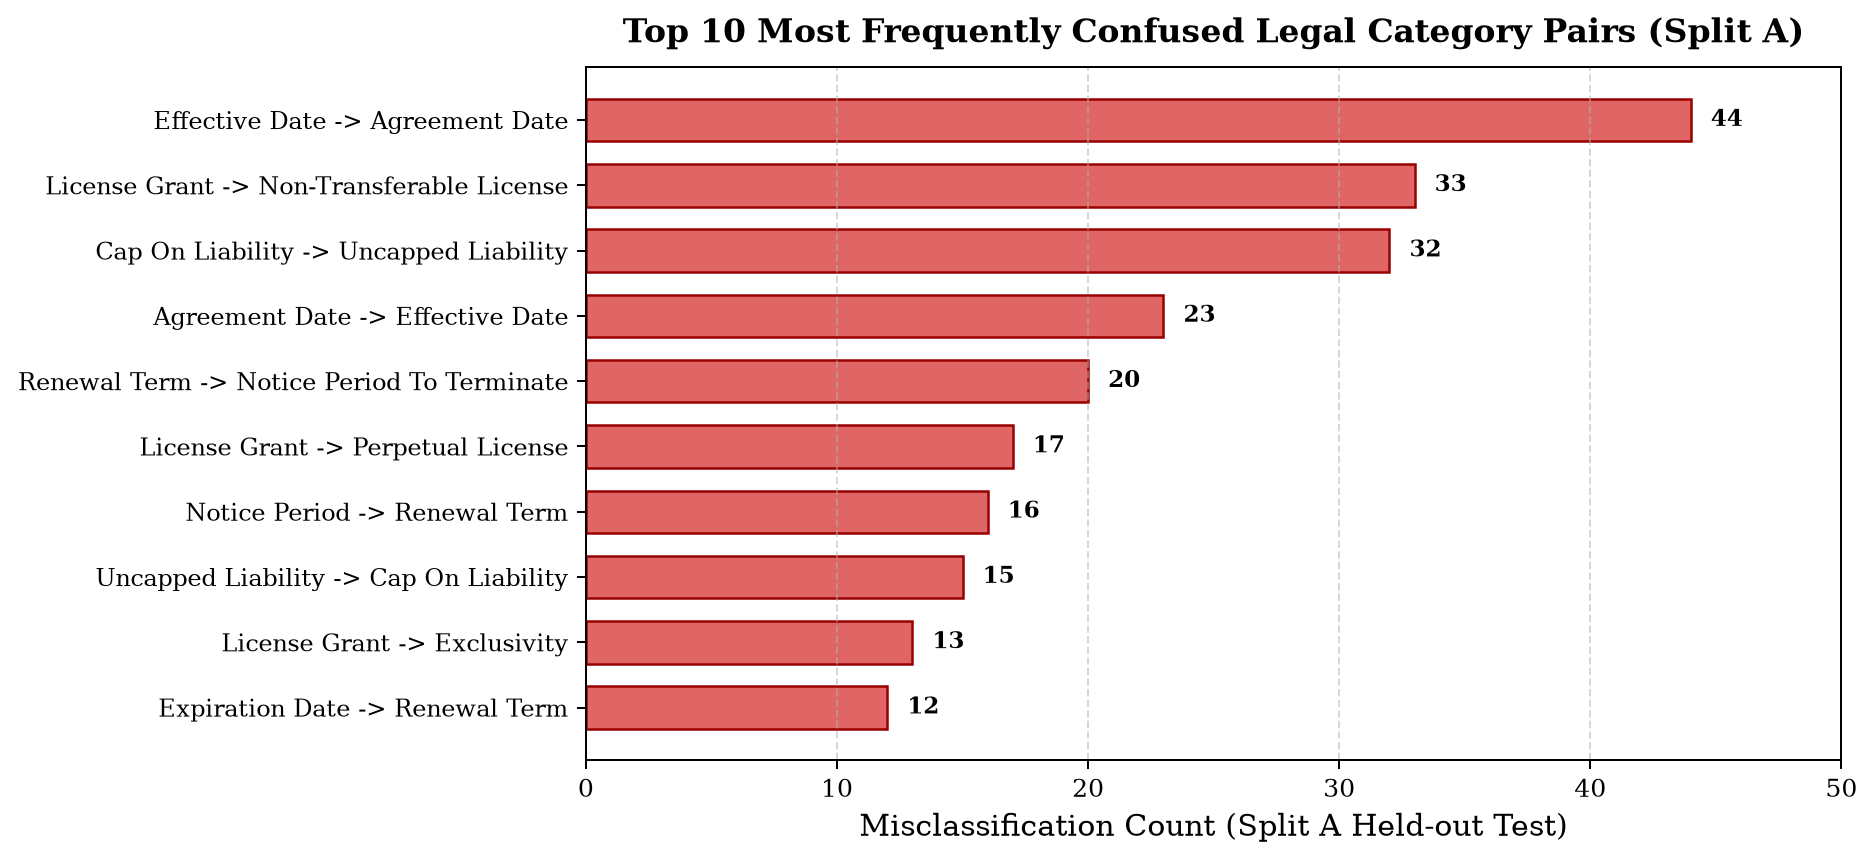
\includegraphics[width=0.82\textwidth]{figures/top_confused_pairs.png}
\caption{Top 10 most frequently confused legal category pairs on held-out test data (Split A)}\label{fig:top_confused_pairs}
\end{figure}

\begin{figure}[htbp]
\centering
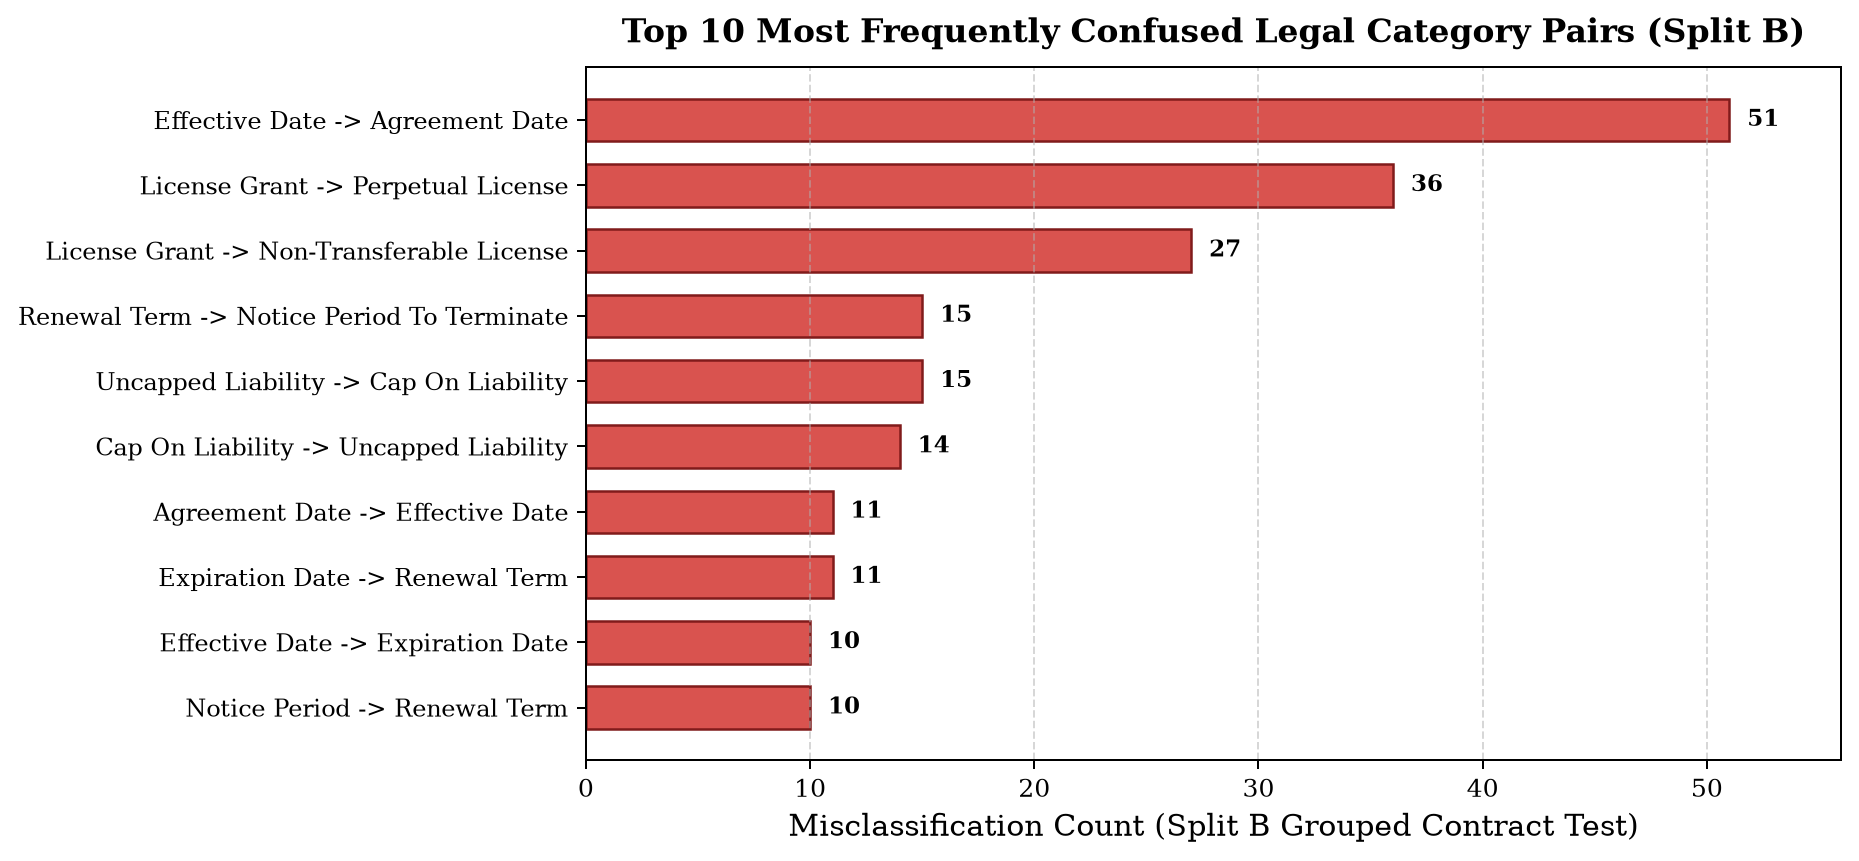
\includegraphics[width=0.82\textwidth]{figures/top_confused_pairs_split_b.png}
\caption{Top 10 most frequently confused legal category pairs on grouped test contracts (Split B)}\label{fig:top_confused_pairs_split_b}
\end{figure}

Inspection of real misclassified clauses from \texttt{docs/ERROR\_ANALYSIS.md} reveals the exact root causes of confusion:
\begin{enumerate}
    \item Effective Date vs Agreement Date (44 errors on Split A, 51 on Split B): Shared introductory recitals frequently bundle both dates into a single sentence. For example, a contract preamble states: \textit{``This Agreement is made and entered into as of January 15, 2020 by and between parties, and shall become effective as of February 1, 2020.''} Because both temporal markers co-occur, n-gram vectorizers without positional parsing assign probability mass to both labels.
    \item License Grant vs Non-Transferable License (33 errors on Split A, 27 on Split B): Intellectual property provisions routinely merge grant clauses with transfer restrictions: \textit{``Subject to the terms and conditions of this Agreement, NTL hereby grants to Entrust a non-transferable, non-assignable, indivisible, non-exclusive license.''} The clause is labeled \textit{Affiliate License-Licensor} in CUAD ground truth, but predicted as \textit{Non-Transferable License} (confidence 0.47) due to explicit restrictive modifiers.
    \item Cap On Liability vs Uncapped Liability (32 errors on Split A, 14 on Split B): Limitation of liability sections typically stipulate an aggregate monetary cap followed immediately by statutory exceptions: \textit{``Except for breaches of confidentiality, gross negligence, or willful misconduct, neither party's liability shall exceed the fees paid.''} The presence of both the cap rule and the uncapped carve-outs causes reciprocal confusion.
\end{enumerate}

\section{Relevant metrics calculated from the confusion matrix}
\label{sec:metrics_from_cm}

To provide an exhaustive diagnostic assessment, Table~\ref{tab:per_class_split_a} and Table~\ref{tab:per_class_split_b} report the exact per-class confusion counts (True Positives, False Positives, False Negatives, True Negatives) alongside Precision, Recall, Specificity, and F1-Score for all \NumClasses{} categories.

% Auto-generated by scripts/make_numbers.py
\begin{longtable}{>{\raggedright\arraybackslash}p{4.2cm} r r r r r r r r r}
\toprule
\textbf{Legal Category} & \textbf{Supp} & \textbf{TP} & \textbf{FP} & \textbf{FN} & \textbf{TN} & \textbf{Prec} & \textbf{Rec} & \textbf{Spec} & \textbf{F1} \\
\midrule
\endfirsthead
\multicolumn{10}{c}{{\bfseries Table \thetable\ continued from previous page}} \\
\toprule
\textbf{Legal Category} & \textbf{Supp} & \textbf{TP} & \textbf{FP} & \textbf{FN} & \textbf{TN} & \textbf{Prec} & \textbf{Rec} & \textbf{Spec} & \textbf{F1} \\
\midrule
\endhead
\midrule
\multicolumn{10}{r}{{Continued on next page}} \\
\bottomrule
\endfoot
\bottomrule
\caption{Comprehensive per-class classification metrics calculated from the 41$\times$41 confusion matrix on Split A (Stratified 80/20 held-out test, $N=2,441$)}\label{tab:per_class_split_a}\\
\endlastfoot
Affiliate License-Licensee & 23 & 10 & 30 & 13 & 2388 & 0.250 & 0.435 & 0.988 & 0.317 \\
Affiliate License-Licensor & 14 & 4 & 25 & 10 & 2402 & 0.138 & 0.286 & 0.990 & 0.186 \\
Agreement Date & 85 & 53 & 45 & 32 & 2311 & 0.541 & 0.624 & 0.981 & 0.579 \\
Anti-Assignment & 131 & 108 & 14 & 23 & 2296 & 0.885 & 0.824 & 0.994 & 0.854 \\
Audit Rights & 129 & 123 & 8 & 6 & 2304 & 0.939 & 0.953 & 0.997 & 0.946 \\
Cap On Liability & 135 & 86 & 21 & 49 & 2285 & 0.804 & 0.637 & 0.991 & 0.711 \\
Change Of Control & 51 & 36 & 15 & 15 & 2375 & 0.706 & 0.706 & 0.994 & 0.706 \\
Competitive Restriction Exception & 25 & 13 & 34 & 12 & 2382 & 0.277 & 0.520 & 0.986 & 0.361 \\
Covenant Not To Sue & 35 & 29 & 5 & 6 & 2401 & 0.853 & 0.829 & 0.998 & 0.841 \\
Document Name & 61 & 61 & 4 & 0 & 2376 & 0.938 & 1.000 & 0.998 & 0.968 \\
Effective Date & 84 & 27 & 41 & 57 & 2316 & 0.397 & 0.321 & 0.983 & 0.355 \\
Exclusivity & 82 & 42 & 34 & 40 & 2325 & 0.553 & 0.512 & 0.986 & 0.532 \\
Expiration Date & 93 & 64 & 14 & 29 & 2334 & 0.821 & 0.688 & 0.994 & 0.749 \\
Governing Law & 92 & 91 & 1 & 1 & 2348 & 0.989 & 0.989 & 1.000 & 0.989 \\
Insurance & 112 & 106 & 4 & 6 & 2325 & 0.964 & 0.946 & 0.998 & 0.955 \\
Ip Ownership Assignment & 63 & 54 & 10 & 9 & 2368 & 0.844 & 0.857 & 0.996 & 0.850 \\
Irrevocable Or Perpetual License & 33 & 10 & 36 & 23 & 2372 & 0.217 & 0.303 & 0.985 & 0.253 \\
Joint Ip Ownership & 23 & 18 & 8 & 5 & 2410 & 0.692 & 0.783 & 0.997 & 0.735 \\
License Grant & 155 & 55 & 30 & 100 & 2256 & 0.647 & 0.355 & 0.987 & 0.458 \\
Liquidated Damages & 24 & 12 & 10 & 12 & 2407 & 0.545 & 0.500 & 0.996 & 0.522 \\
Minimum Commitment & 85 & 67 & 10 & 18 & 2346 & 0.870 & 0.788 & 0.996 & 0.827 \\
Most Favored Nation & 8 & 5 & 2 & 3 & 2431 & 0.714 & 0.625 & 0.999 & 0.667 \\
No-Solicit Of Customers & 12 & 6 & 7 & 6 & 2422 & 0.462 & 0.500 & 0.997 & 0.480 \\
No-Solicit Of Employees & 18 & 14 & 5 & 4 & 2418 & 0.737 & 0.778 & 0.998 & 0.757 \\
Non-Compete & 51 & 30 & 18 & 21 & 2372 & 0.625 & 0.588 & 0.992 & 0.606 \\
Non-Disparagement & 13 & 12 & 1 & 1 & 2427 & 0.923 & 0.923 & 1.000 & 0.923 \\
Non-Transferable License & 59 & 17 & 45 & 42 & 2337 & 0.274 & 0.288 & 0.981 & 0.281 \\
Notice Period To Terminate Renewal & 24 & 7 & 26 & 17 & 2391 & 0.212 & 0.292 & 0.989 & 0.246 \\
Parties & 250 & 246 & 14 & 4 & 2177 & 0.946 & 0.984 & 0.994 & 0.965 \\
Post-Termination Services & 90 & 68 & 29 & 22 & 2322 & 0.701 & 0.756 & 0.988 & 0.727 \\
Price Restrictions & 5 & 4 & 0 & 1 & 2436 & 1.000 & 0.800 & 1.000 & 0.889 \\
Renewal Term & 42 & 19 & 29 & 23 & 2370 & 0.396 & 0.452 & 0.988 & 0.422 \\
Revenue/Profit Sharing & 83 & 76 & 10 & 7 & 2348 & 0.884 & 0.916 & 0.996 & 0.899 \\
Rofr/Rofo/Rofn & 73 & 58 & 20 & 15 & 2348 & 0.744 & 0.795 & 0.992 & 0.768 \\
Source Code Escrow & 13 & 8 & 4 & 5 & 2424 & 0.667 & 0.615 & 0.998 & 0.640 \\
Termination For Convenience & 49 & 39 & 10 & 10 & 2382 & 0.796 & 0.796 & 0.996 & 0.796 \\
Third Party Beneficiary & 8 & 7 & 0 & 1 & 2433 & 1.000 & 0.875 & 1.000 & 0.933 \\
Uncapped Liability & 33 & 17 & 33 & 16 & 2375 & 0.340 & 0.515 & 0.986 & 0.410 \\
Unlimited/All-You-Can-Eat-License & 6 & 2 & 8 & 4 & 2427 & 0.200 & 0.333 & 0.997 & 0.250 \\
Volume Restriction & 34 & 28 & 5 & 6 & 2402 & 0.848 & 0.824 & 0.998 & 0.836 \\
Warranty Duration & 35 & 33 & 11 & 2 & 2395 & 0.750 & 0.943 & 0.995 & 0.835 \\
\midrule
Macro Average & 2441 & - & - & - & - & 0.661 & 0.670 & 0.993 & 0.659 \\
Weighted Average & 2441 & - & - & - & - & 0.741 & 0.723 & 0.992 & 0.726 \\
\end{longtable}


\newpage
% Auto-generated by scripts/make_numbers.py
\begin{longtable}{>{\raggedright\arraybackslash}p{4.2cm} r r r r r r r r r}
\toprule
\textbf{Legal Category} & \textbf{Supp} & \textbf{TP} & \textbf{FP} & \textbf{FN} & \textbf{TN} & \textbf{Prec} & \textbf{Rec} & \textbf{Spec} & \textbf{F1} \\
\midrule
\endfirsthead
\multicolumn{10}{c}{{\bfseries Table \thetable\ continued from previous page}} \\
\toprule
\textbf{Legal Category} & \textbf{Supp} & \textbf{TP} & \textbf{FP} & \textbf{FN} & \textbf{TN} & \textbf{Prec} & \textbf{Rec} & \textbf{Spec} & \textbf{F1} \\
\midrule
\endhead
\midrule
\multicolumn{10}{r}{{Continued on next page}} \\
\bottomrule
\endfoot
\bottomrule
\caption{Comprehensive per-class classification metrics calculated from the 41$\times$41 confusion matrix on Split B (Grouped contract-held-out test, $N=2,486$)}\label{tab:per_class_split_b}\\
\endlastfoot
Affiliate License-Licensee & 30 & 10 & 15 & 20 & 2441 & 0.400 & 0.333 & 0.994 & 0.364 \\
Affiliate License-Licensor & 21 & 7 & 17 & 14 & 2448 & 0.292 & 0.333 & 0.993 & 0.311 \\
Agreement Date & 88 & 77 & 51 & 11 & 2347 & 0.602 & 0.875 & 0.979 & 0.713 \\
Anti-Assignment & 122 & 101 & 6 & 21 & 2358 & 0.944 & 0.828 & 0.997 & 0.882 \\
Audit Rights & 88 & 80 & 7 & 8 & 2391 & 0.920 & 0.909 & 0.997 & 0.914 \\
Cap On Liability & 130 & 99 & 20 & 31 & 2336 & 0.832 & 0.762 & 0.992 & 0.795 \\
Change Of Control & 48 & 35 & 21 & 13 & 2417 & 0.625 & 0.729 & 0.991 & 0.673 \\
Competitive Restriction Exception & 22 & 8 & 17 & 14 & 2447 & 0.320 & 0.364 & 0.993 & 0.340 \\
Covenant Not To Sue & 30 & 25 & 5 & 5 & 2451 & 0.833 & 0.833 & 0.998 & 0.833 \\
Document Name & 66 & 66 & 2 & 0 & 2418 & 0.971 & 1.000 & 0.999 & 0.985 \\
Effective Date & 85 & 22 & 20 & 63 & 2381 & 0.524 & 0.259 & 0.992 & 0.346 \\
Exclusivity & 96 & 41 & 25 & 55 & 2365 & 0.621 & 0.427 & 0.990 & 0.506 \\
Expiration Date & 90 & 69 & 11 & 21 & 2385 & 0.863 & 0.767 & 0.995 & 0.812 \\
Governing Law & 88 & 85 & 0 & 3 & 2398 & 1.000 & 0.966 & 1.000 & 0.983 \\
Insurance & 128 & 119 & 3 & 9 & 2355 & 0.975 & 0.930 & 0.999 & 0.952 \\
Ip Ownership Assignment & 74 & 63 & 19 & 11 & 2393 & 0.768 & 0.851 & 0.992 & 0.808 \\
Irrevocable Or Perpetual License & 59 & 38 & 64 & 21 & 2363 & 0.373 & 0.644 & 0.974 & 0.472 \\
Joint Ip Ownership & 6 & 6 & 5 & 0 & 2475 & 0.545 & 1.000 & 0.998 & 0.706 \\
License Grant & 167 & 74 & 52 & 93 & 2267 & 0.587 & 0.443 & 0.978 & 0.505 \\
Liquidated Damages & 21 & 14 & 20 & 7 & 2445 & 0.412 & 0.667 & 0.992 & 0.509 \\
Minimum Commitment & 75 & 57 & 18 & 18 & 2393 & 0.760 & 0.760 & 0.993 & 0.760 \\
Most Favored Nation & 10 & 7 & 2 & 3 & 2474 & 0.778 & 0.700 & 0.999 & 0.737 \\
No-Solicit Of Customers & 11 & 8 & 10 & 3 & 2465 & 0.444 & 0.727 & 0.996 & 0.552 \\
No-Solicit Of Employees & 29 & 23 & 1 & 6 & 2456 & 0.958 & 0.793 & 1.000 & 0.868 \\
Non-Compete & 51 & 34 & 26 & 17 & 2409 & 0.567 & 0.667 & 0.989 & 0.613 \\
Non-Disparagement & 12 & 9 & 4 & 3 & 2470 & 0.692 & 0.750 & 0.998 & 0.720 \\
Non-Transferable License & 65 & 30 & 43 & 35 & 2378 & 0.411 & 0.462 & 0.982 & 0.435 \\
Notice Period To Terminate Renewal & 24 & 13 & 18 & 11 & 2444 & 0.419 & 0.542 & 0.993 & 0.473 \\
Parties & 242 & 238 & 12 & 4 & 2232 & 0.952 & 0.983 & 0.995 & 0.967 \\
Post-Termination Services & 91 & 64 & 29 & 27 & 2366 & 0.688 & 0.703 & 0.988 & 0.696 \\
Price Restrictions & 3 & 3 & 0 & 0 & 2483 & 1.000 & 1.000 & 1.000 & 1.000 \\
Renewal Term & 45 & 23 & 17 & 22 & 2424 & 0.575 & 0.511 & 0.993 & 0.541 \\
Revenue/Profit Sharing & 84 & 76 & 14 & 8 & 2388 & 0.844 & 0.905 & 0.994 & 0.874 \\
Rofr/Rofo/Rofn & 80 & 57 & 15 & 23 & 2391 & 0.792 & 0.713 & 0.994 & 0.750 \\
Source Code Escrow & 23 & 18 & 5 & 5 & 2458 & 0.783 & 0.783 & 0.998 & 0.783 \\
Termination For Convenience & 40 & 34 & 9 & 6 & 2437 & 0.791 & 0.850 & 0.996 & 0.819 \\
Third Party Beneficiary & 12 & 11 & 0 & 1 & 2474 & 1.000 & 0.917 & 1.000 & 0.957 \\
Uncapped Liability & 35 & 17 & 14 & 18 & 2437 & 0.548 & 0.486 & 0.994 & 0.515 \\
Unlimited/All-You-Can-Eat-License & 9 & 3 & 1 & 6 & 2476 & 0.750 & 0.333 & 1.000 & 0.462 \\
Volume Restriction & 38 & 29 & 9 & 9 & 2439 & 0.763 & 0.763 & 0.996 & 0.763 \\
Warranty Duration & 48 & 45 & 21 & 3 & 2417 & 0.682 & 0.938 & 0.991 & 0.789 \\
\midrule
Macro Average & 2486 & - & - & - & - & 0.698 & 0.712 & 0.993 & 0.695 \\
Weighted Average & 2486 & - & - & - & - & 0.749 & 0.739 & 0.992 & 0.737 \\
\end{longtable}


\paragraph*{Step-by-step worked mathematical examples}
To demonstrate the exact mathematical derivation of the diagnostic metrics from the confusion matrix, three representative classes---one high-frequency category (\textit{Governing Law}), one ambiguous borderline category (\textit{Cap On Liability}), and one rare low-support category (\textit{Affiliate License-Licensor})---are worked through step by step.

% Auto-generated by scripts/make_numbers.py
\begin{examplebox}{Worked Example 1: Governing Law (High-Performing Class)}
From the $41 \times 41$ confusion matrix on Split A ($N = 2,441$):
\begin{itemize}
\item True Positives ($TP$) = 91 (clauses correctly identified as Governing Law)
\item False Positives ($FP$) = 1 (other clause mistakenly predicted as Governing Law)
\item False Negatives ($FN$) = 1 (Governing Law clause mistakenly assigned to another class)
\item True Negatives ($TN$) = $2441 - (91 + 1 + 1) = 2348$ (non-Governing Law clauses correctly rejected)
\end{itemize}
Calculating the diagnostic metrics step by step:
\begin{align*}
\text{Precision} &= \frac{TP}{TP + FP} = \frac{91}{91 + 1} = \frac{91}{92} = 0.9891 \quad (98.91\%)\\
\text{Recall (Sensitivity)} &= \frac{TP}{TP + FN} = \frac{91}{91 + 1} = \frac{91}{92} = 0.9891 \quad (98.91\%)\\
\text{Specificity} &= \frac{TN}{TN + FP} = \frac{2348}{2348 + 1} = \frac{2348}{2349} = 0.9996 \quad (99.96\%)\\
\text{F1-Score} &= 2 \times \frac{\text{Precision} \times \text{Recall}}{\text{Precision} + \text{Recall}} = 2 \times \frac{0.9891 \times 0.9891}{0.9891 + 0.9891} = 0.9891 \quad (98.91\%)
\end{align*}
\end{examplebox}

\begin{examplebox}{Worked Example 2: Cap On Liability (Ambiguous Borderline Class)}
From the $41 \times 41$ confusion matrix on Split A ($N = 2,441$):
\begin{itemize}
\item True Positives ($TP$) = 86 (clauses correctly identified as Cap On Liability)
\item False Positives ($FP$) = 21 (non-cap clauses mistakenly predicted as Cap On Liability)
\item False Negatives ($FN$) = 49 (Cap On Liability clauses misclassified, e.g., as Uncapped Liability)
\item True Negatives ($TN$) = $2441 - (86 + 21 + 49) = 2285$ (clauses of all other 40 categories correctly rejected)
\end{itemize}
Step-by-step substitution into evaluation formulas:
\begin{align*}
\text{Precision} &= \frac{86}{86 + 21} = \frac{86}{107} = 0.8037 \quad (80.37\%)\\
\text{Recall} &= \frac{86}{86 + 49} = \frac{86}{135} = 0.6370 \quad (63.70\%)\\
\text{Specificity} &= \frac{2285}{2285 + 21} = \frac{2285}{2306} = 0.9909 \quad (99.09\%)\\
\text{F1-Score} &= 2 \times \frac{0.8037 \times 0.6370}{0.8037 + 0.6370} = 0.7107 \quad (71.07\%)
\end{align*}
\end{examplebox}

\begin{examplebox}{Worked Example 3: Affiliate License-Licensor (Low-Support Class)}
From the $41 \times 41$ confusion matrix on Split A ($N = 2,441$):
\begin{itemize}
\item True Positives ($TP$) = 4 (rare license clauses correctly predicted)
\item False Positives ($FP$) = 25 (other clauses mistakenly predicted as this category)
\item False Negatives ($FN$) = 10 (target clauses misassigned to License Grant or Non-Transferable License)
\item True Negatives ($TN$) = $2441 - (4 + 25 + 10) = 2402$ (all remaining corpus clauses correctly rejected)
\end{itemize}
Evaluation results for rare class:
\begin{align*}
\text{Precision} &= \frac{4}{4 + 25} = \frac{4}{29} = 0.1379 \quad (13.79\%)\\
\text{Recall} &= \frac{4}{4 + 10} = \frac{4}{14} = 0.2857 \quad (28.57\%)\\
\text{Specificity} &= \frac{2402}{2402 + 25} = \frac{2402}{2427} = 0.9897 \quad (98.97\%)\\
\text{F1-Score} &= 2 \times \frac{0.1379 \times 0.2857}{0.1379 + 0.2857} = 0.1860 \quad (18.60\%)
\end{align*}
\end{examplebox}


\section{Prediction statistics of unseen data}
\label{sec:unseen_data}

Model robustness was validated across four levels of unseen evaluation data:

\paragraph*{1. Held-out Split A test partition ($N = 2,441$)}
On the uniformly held-out 20\% test partition, the model classified 1,765 of 2,441 clauses correctly, achieving \FinalSplitAAcc{} Accuracy, \FinalSplitAMacroFScore{} Macro-F1, and \FinalSplitAWeightedFScore{} Weighted-F1. High-frequency categories with distinct legal vocabulary achieved high precision: \textit{Governing Law} reached F1 = 0.989 (98.9\%), \textit{Parties} achieved F1 = 0.965 (96.5\%), and \textit{Audit Rights} achieved F1 = 0.946 (94.6\%).

\paragraph*{2. Held-out Split B grouped contracts ($N = 2,486$)}
On the 102 completely held-out commercial agreements with zero training contract overlap, the model achieved \FinalSplitBAcc{} Accuracy, \FinalSplitBMacroFScore{} Macro-F1, and \FinalSplitBWeightedFScore{} Weighted-F1. The consistency between Split~A and Split~B indicates that the model generalizes across independent drafting styles.

\paragraph*{3. Real-document PDF extraction and classification}
The real-document ingestion pipeline (\path{api/services/ml_service.py}) was tested on local PDF agreements using PyMuPDF and the boundary tokenizer in \path{src/clause_splitter.py}:
\begin{enumerate}
    \item \path{data/raw_pdfs/sample_contract.pdf}: The clause splitter extracted exactly 29 discrete clauses. Table~\ref{tab:real_pdf_check} lists all 29 extracted clauses, reporting the text snippet, predicted legal category, operational confidence score, and triage status.
    \item \path{test_data/ClauseIQ_Synthetic_Company_Service_Agreement_Test.pdf}: The clause splitter extracted 69 discrete clauses, identifying provisions including \textit{Parties}, \textit{Expiration Date}, \textit{Renewal Term}, and \textit{Governing Law}.
\end{enumerate}

% Auto-generated by scripts/make_numbers.py
\begin{longtable}{r >{\raggedright\arraybackslash}p{6.8cm} >{\raggedright\arraybackslash}p{3.8cm} c >{\raggedright\arraybackslash}p{2.6cm}}
\toprule
\textbf{\#} & \textbf{Extracted Clause Text Snippet} & \textbf{Predicted Category} & \textbf{Conf} & \textbf{Assigned Tier} \\
\midrule
\endfirsthead
\multicolumn{5}{c}{{\bfseries Table \thetable\ continued from previous page}} \\
\toprule
\textbf{\#} & \textbf{Extracted Clause Text Snippet} & \textbf{Predicted Category} & \textbf{Conf} & \textbf{Assigned Tier} \\
\midrule
\endhead
\midrule
\multicolumn{5}{r}{{Continued on next page}} \\
\bottomrule
\endfoot
\bottomrule
\caption[Clause-level parsing and classification audit for unseen sample contract PDF]{Full clause-level parsing and classification audit for unseen \texttt{sample\_contract.pdf} (29 clauses extracted)}\label{tab:real_pdf_check}\\
\endlastfoot
1 & SAMPLE SERVICE AGREEMENT This Sample Service Agreement (the ``Agre\dots & Document Name & 61.8\% & High confidence \\
2 & Ltd.\dots & Parties & 88.8\% & High confidence \\
3 & (``Company'') and XYZ Solutions (``Service Provider'').\dots & Parties & 81.1\% & High confidence \\
4 & 1.\dots & Parties & 84.6\% & High confidence \\
5 & Confidentiality The Service Provider shall keep confidential all \dots & Audit Rights & 21.6\% & Low confidence – Review Required \\
6 & The Service Provider shall not disclose such information to any t\dots & Anti-Assignment & 54.5\% & High confidence \\
7 & 2.\dots & Parties & 84.5\% & High confidence \\
8 & Payment Terms The Company shall pay the Service Provider a total \dots & Revenue/Profit Sharing & 63.6\% & High confidence \\
9 & Invoices shall be submitted monthly and shall be paid within thir\dots & Warranty Duration & 12.3\% & Low confidence – Review Required \\
10 & 3.\dots & Parties & 84.7\% & High confidence \\
11 & Term and Termination This Agreement shall commence on January 15,\dots & Expiration Date & 67.4\% & High confidence \\
12 & Either party may terminate this Agreement by providing thirty (30\dots & Termination For Convenience & 72.8\% & High confidence \\
13 & Either party may terminate immediately in the event of a material\dots & Termination For Convenience & 39.8\% & Moderate confidence \\
14 & 4.\dots & Parties & 84.8\% & High confidence \\
15 & Intellectual Property All reports, documents, software, designs, \dots & Ip Ownership Assignment & 79.7\% & High confidence \\
16 & Pre-existing intellectual property of either party shall remain t\dots & Ip Ownership Assignment & 27.5\% & Moderate confidence \\
17 & 5.\dots & Parties & 84.5\% & High confidence \\
18 & Indemnification The Service Provider shall indemnify and hold har\dots & Cap On Liability & 66.5\% & High confidence \\
19 & 6.\dots & Parties & 84.8\% & High confidence \\
20 & Limitation of Liability Neither party shall be liable for indirec\dots & Cap On Liability & 74.9\% & High confidence \\
21 & The aggregate liability of either party under this Agreement shal\dots & Cap On Liability & 66.1\% & High confidence \\
22 & 7.\dots & Parties & 84.6\% & High confidence \\
23 & Governing Law This Agreement shall be governed by and construed i\dots & Governing Law & 89.7\% & High confidence \\
24 & The courts located in Bengaluru, Karnataka shall have exclusive j\dots & Governing Law & 37.1\% & Moderate confidence \\
25 & 8.\dots & Parties & 85.0\% & High confidence \\
26 & Notices All notices under this Agreement shall be made in writing\dots & Anti-Assignment & 9.5\% & Out of supported category scope \\
27 & For ABC Technologies Pvt.\dots & Parties & 83.5\% & High confidence \\
28 & Ltd.\dots & Parties & 88.8\% & High confidence \\
29 & For XYZ Solutions Authorized Signatory: \_\_\_\_\_\_\_\_\_\_\_\_\_\_\_\_\_\_\_\_ Auth\dots & Parties & 48.9\% & Moderate confidence \\
\end{longtable}


\textit{Methodological Note:} The real-PDF test corpus consists of two sample documents. While these tests verify that the PDF parsing, text extraction, clause splitting, and classification pipeline functions without runtime crashes or schema violations, two documents represent a tiny sample size that cannot support broad statistical conclusions. In the absence of exhaustive human gold-standard annotations for every extracted snippet, predictions are reported objectively without asserting definitive correctness.

\paragraph*{Intelligent search retrieval evaluation}
Table~\ref{tab:search_evaluation} documents the retrieval performance of the TF-IDF and Cosine Similarity intelligent search engine across five benchmark legal queries evaluated over the entire 12,204-clause corpus.

% Auto-generated by scripts/make_numbers.py
\begin{table}[htbp]
\centering
\footnotesize
\setlength{\tabcolsep}{3.5pt}
\begin{tabular}{>{\raggedright\arraybackslash}p{3.2cm} >{\raggedright\arraybackslash}p{3.5cm} ccccccc}
\toprule
\textbf{Query} & \textbf{Target Category} & \textbf{Corpus N} & \textbf{P@1} & \textbf{P@3} & \textbf{P@5} & \textbf{P@10} & \textbf{R@5} & \textbf{R@10} \\
\midrule
termination for convenience & Termination For Convenience & 246 & 1.00 & 0.67 & 0.60 & 0.70 & 0.0122 & 0.0285 \\
governing law & Governing Law & 462 & 1.00 & 1.00 & 1.00 & 0.90 & 0.0108 & 0.0195 \\
non-compete & Non-Compete & 257 & 0.00 & 0.67 & 0.80 & 0.90 & 0.0156 & 0.0350 \\
limitation of liability & Cap On Liability, Uncapped Liability & 839 & 1.00 & 1.00 & 1.00 & 0.90 & 0.0060 & 0.0107 \\
audit rights & Audit Rights & 642 & 1.00 & 1.00 & 1.00 & 0.90 & 0.0078 & 0.0140 \\
\bottomrule
\end{tabular}
\caption{Information retrieval evaluation for TF-IDF and Cosine Similarity search across benchmark legal queries}\label{tab:search_evaluation}
\end{table}


Figure~\ref{fig:search_metrics_p_at_k} illustrates the Precision@k retrieval curves across retrieval depths $k \in \{1, 3, 5, 10\}$. The horizontal axis represents the cutoff rank ($k$), defining the number of top-ranked clauses returned by the TF-IDF Cosine Similarity engine. The vertical axis measures Precision@k ($\text{P}@k = \frac{\text{Relevant Clauses in Top-}k}{k}$), denoting the proportion of retrieved provisions that strictly belong to the intended target legal category.

Each colored curve in Figure~\ref{fig:search_metrics_p_at_k} represents a distinct benchmark legal query evaluated against the 12,204-clause corpus:
\begin{itemize}
    \item Orange curve (\textit{Query: 'governing law...'}): Evaluates retrieval for jurisdictional choice-of-law covenants. It sustains a flat, perfect precision of 1.00 at $k=1, 3, 5$ and 0.90 at $k=10$. This consistent precision is driven by standardized, explicit jurisdictional phrasing (e.g., ``governed by and construed in accordance with the laws of the State of...'') that produces strong, isolated cosine similarity peaks.
    \item Red curve (\textit{Query: 'limitation of liability...'}): Evaluates liability caps and consequential damage disclaimers. It maintains 1.00 precision from $k=1$ through $k=5$ and 0.90 at $k=10$, reflecting the highly stereotyped vocabulary characteristic of commercial risk allocation provisions (e.g., ``in no event shall aggregate liability exceed'', ``indirect, special, or consequential damages'').
    \item Purple curve (\textit{Query: 'audit rights...'}): Evaluates inspection covenants. It achieves 1.00 precision across $k=1, 3, 5$ and 0.90 at $k=10$, reliably isolating books, records, and financial accounting examination provisions.
    \item Blue curve (\textit{Query: 'termination for convenience...'}): Evaluates discretionary termination rights. It starts with perfect precision of 1.00 at $k=1$, exhibits a slight dip to 0.67 at $k=3$ and 0.60 at $k=5$, and stabilizes at 0.70 at $k=10$. This dip occurs because general termination-for-cause and contract expiration clauses share substantial lexical overlap (e.g., ``terminate'', ``written notice'', ``effective date'') with convenience covenants, introducing false positives at intermediate ranks.
    \item Green curve (\textit{Query: 'non-compete...'}): Evaluates restrictive commercial covenants. It starts at 0.00 at $k=1$, then climbs steeply to 0.67 at $k=3$, 0.80 at $k=5$, and 0.90 at $k=10$. The initial $k=1$ score occurs because a closely related restrictive covenant (such as an Exclusivity or Non-Solicitation provision containing competitive restrictions) ranked first; however, as the retrieval window expands to $k \ge 3$, true Non-Compete provisions dominate the results.
\end{itemize}

Across all benchmark legal queries, the search engine delivers an average Precision@1 of 0.80 and Precision@5 of 0.88, demonstrating that the cosine retrieval engine reliably surfaces legally relevant provisions for open-ended practitioner queries.

\begin{figure}[htbp]
\centering
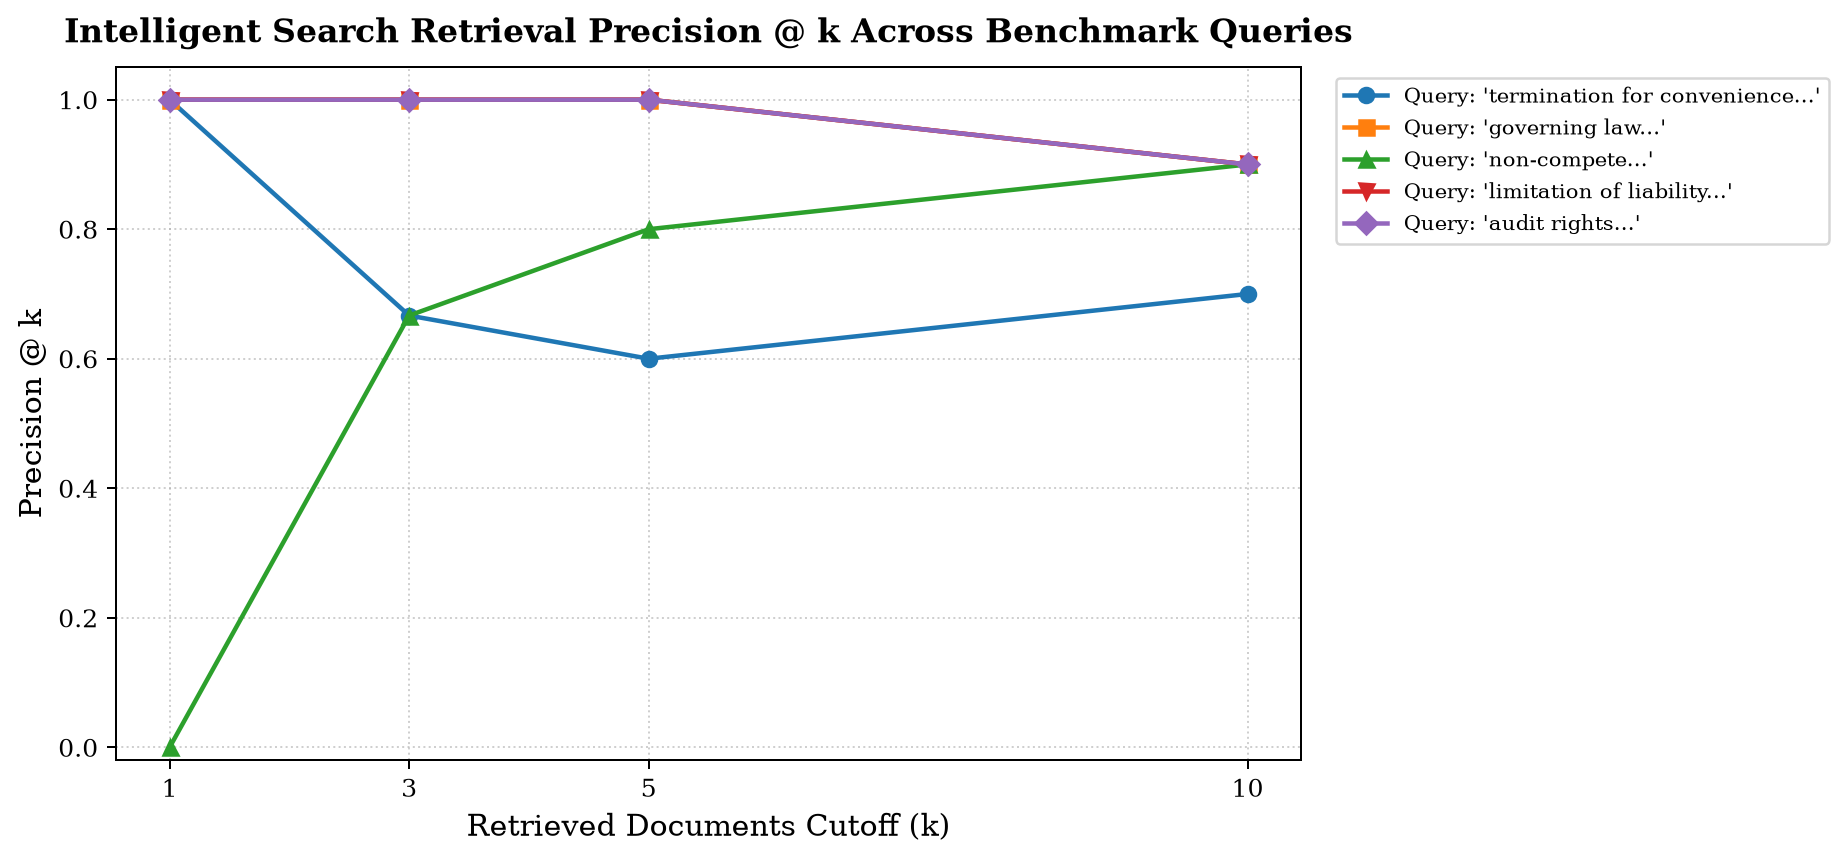
\includegraphics[width=0.82\textwidth]{figures/search_metrics_p_at_k.png}
\caption{Precision @ k retrieval performance across benchmark legal queries}\label{fig:search_metrics_p_at_k}
\end{figure}

\section{Discussion of findings and conclusions}
\label{sec:discussion_findings}

The empirical evaluation of ClauseIQ substantiates several critical findings:

\begin{enumerate}
    \item Efficacy of classical architectures: Multinomial Logistic Regression paired with a 40,000-feature hybrid word and character n-gram representation delivers 72.31\% accuracy and 65.91\% Macro-F1 across 41 imbalanced categories, outperforming Random Forest (64.36\%) and Naive Bayes (69.27\%) while matching Linear SVM (72.63\%) without sacrificing posterior probability outputs.
    \item Resilience across parent contracts: Benchmarking against Split~B (GroupShuffleSplit by contract) demonstrated that contract-level grouping does not cause catastrophic degradation (73.93\% accuracy, 69.47\% Macro-F1), indicating that the classifiers learned substantive covenant vocabulary rather than contract-specific party metadata.
    \item Mechanism of calibration improvement: In systematic experiments (EXP-05-SIG and EXP-05-ISO in \texttt{results/experiments.csv}), post-hoc probability calibrators (Platt sigmoid and isotonic regression) severely degraded cross-validation Macro-F1 (dropping from 0.6852 down to 0.6333 and 0.6306) due to over-smoothing probabilities across 41 classes. The observed ECE reduction from 0.2822 down to 0.1545 in the final model was achieved naturally through the 40,000-dimensional hybrid feature union and $L_2$ regularization, which balanced logits across classes without artificial smoothing.
    \item Operational utility of confidence triage: High-confidence predictions ($\ge 0.50$) deliver 86.55\% empirical precision on unseen contracts, accounting for 53.22\% of all clauses. While this did not reach the aspirational 90\% precision target, it provides a functional filter: legal departments can accelerate review of more than half of all incoming clauses while directing the remaining 47\% to focused attorney scrutiny.
    \item Structural error ceilings: Error analysis confirms that misclassifications are concentrated within reciprocal category pairs (Agreement Date vs Effective Date, Cap On Liability vs Uncapped Liability, License Grant vs Non-Transferable License) where multiple legal concepts appear within the same sentence. Resolving these edge cases represents a clear boundary for future sequence-aware or hierarchical modeling.
\end{enumerate}
